\chapter{Implementation and discussion} \label{chap: Result}

In order to verify the feasibility of the methodologies from chapter \ref{chap: Meth}, 
performance testing based on assumptions and two industrial uses cases 
are done and their results will be performed and discussed in this chapter. 
Again, the tests will also be divided into internal (\ref{chap: Result-Internal}) 
and external (\ref{chap: Result-External}) part, referring to those in chapter \ref{chap: Meth}.

\section{Internal}\label{chap: Result-Internal}
For the internal \gls{mas}, multiple tests are performed on the agent 
communication system. That means, the messages 
will be passed through the \gls{ca} under WebSocket architecture. 
Various tests will be done and the test results will be discussed later in section 
\ref{chap: Result-WS}. 
In addition to the performance testing of WebSocket architecture alone, 
a comparison between WebSocket and \gls{http} will be done to verify the feasibility 
of WebSocket. 
After that, tests relevant to packets prioritization will be performed in 
section \ref{chap: Result-priority}. 
Finally, tests results of the WebSocket based \gls{mas} architecture under 
BMW use case will be presented to close the sections.


\subsection{Test results of WebSocket in various performance testing including worst case scenarios} \label{chap: Result-WS}

After the construction a \gls{mas} under WebSocket, the speed, robustness, 
reliability and application size of the system will be examined by 
performance tests. 

\subsubsection{Increasing client numbers}
In real world, the number of clients will greatly influence the performance of 
server. Assume that all agents serve as clients and \gls{ca} as a central server. 
  

By handling an increasing number of connection requests, and the growing demands 
of data processing capacity, the average total delay with or without process time can be 
roughly described as an overall increasing pattern. However, it does not necessarily 
need to be linear based on several reasons. In exercise, concurrent programming 
will speed up the processing for a large computation problem. As depicted in 
fig.\ref{fig: proportional-clients}, the average process time from one to ten 
clients is decreasing with a better utilization of the CPU power due to 
concurrent processing. However, by further increasing the clients number, the 
speedup will be limited by CPU cores number. Assume that a CPU has 8 core, 
and each core can handle 2 threads, it will have in total 16 threads to perform tasks.
In WebSocket based \gls{mas} program, the asynchronous I/O framework asyncio is used 
to handle the coroutines execution in order to better utilize the threads power.
Therefore, the asyncio is potentially more suitable for larger computational tasks 
compared to synchronous single thread programming.

Obviously there is a limit of the clients number to prevent system breakdown. 
With one server handling all clients at once, there is a system timeout problem of 
the server when the clients number reaches 1000. Therefore, 
distributing clients with more servers becomes a possible solution. 


\begin{figure}[htb]
    \begin{subfigure}[b]{0.49\textwidth}
        \centering
        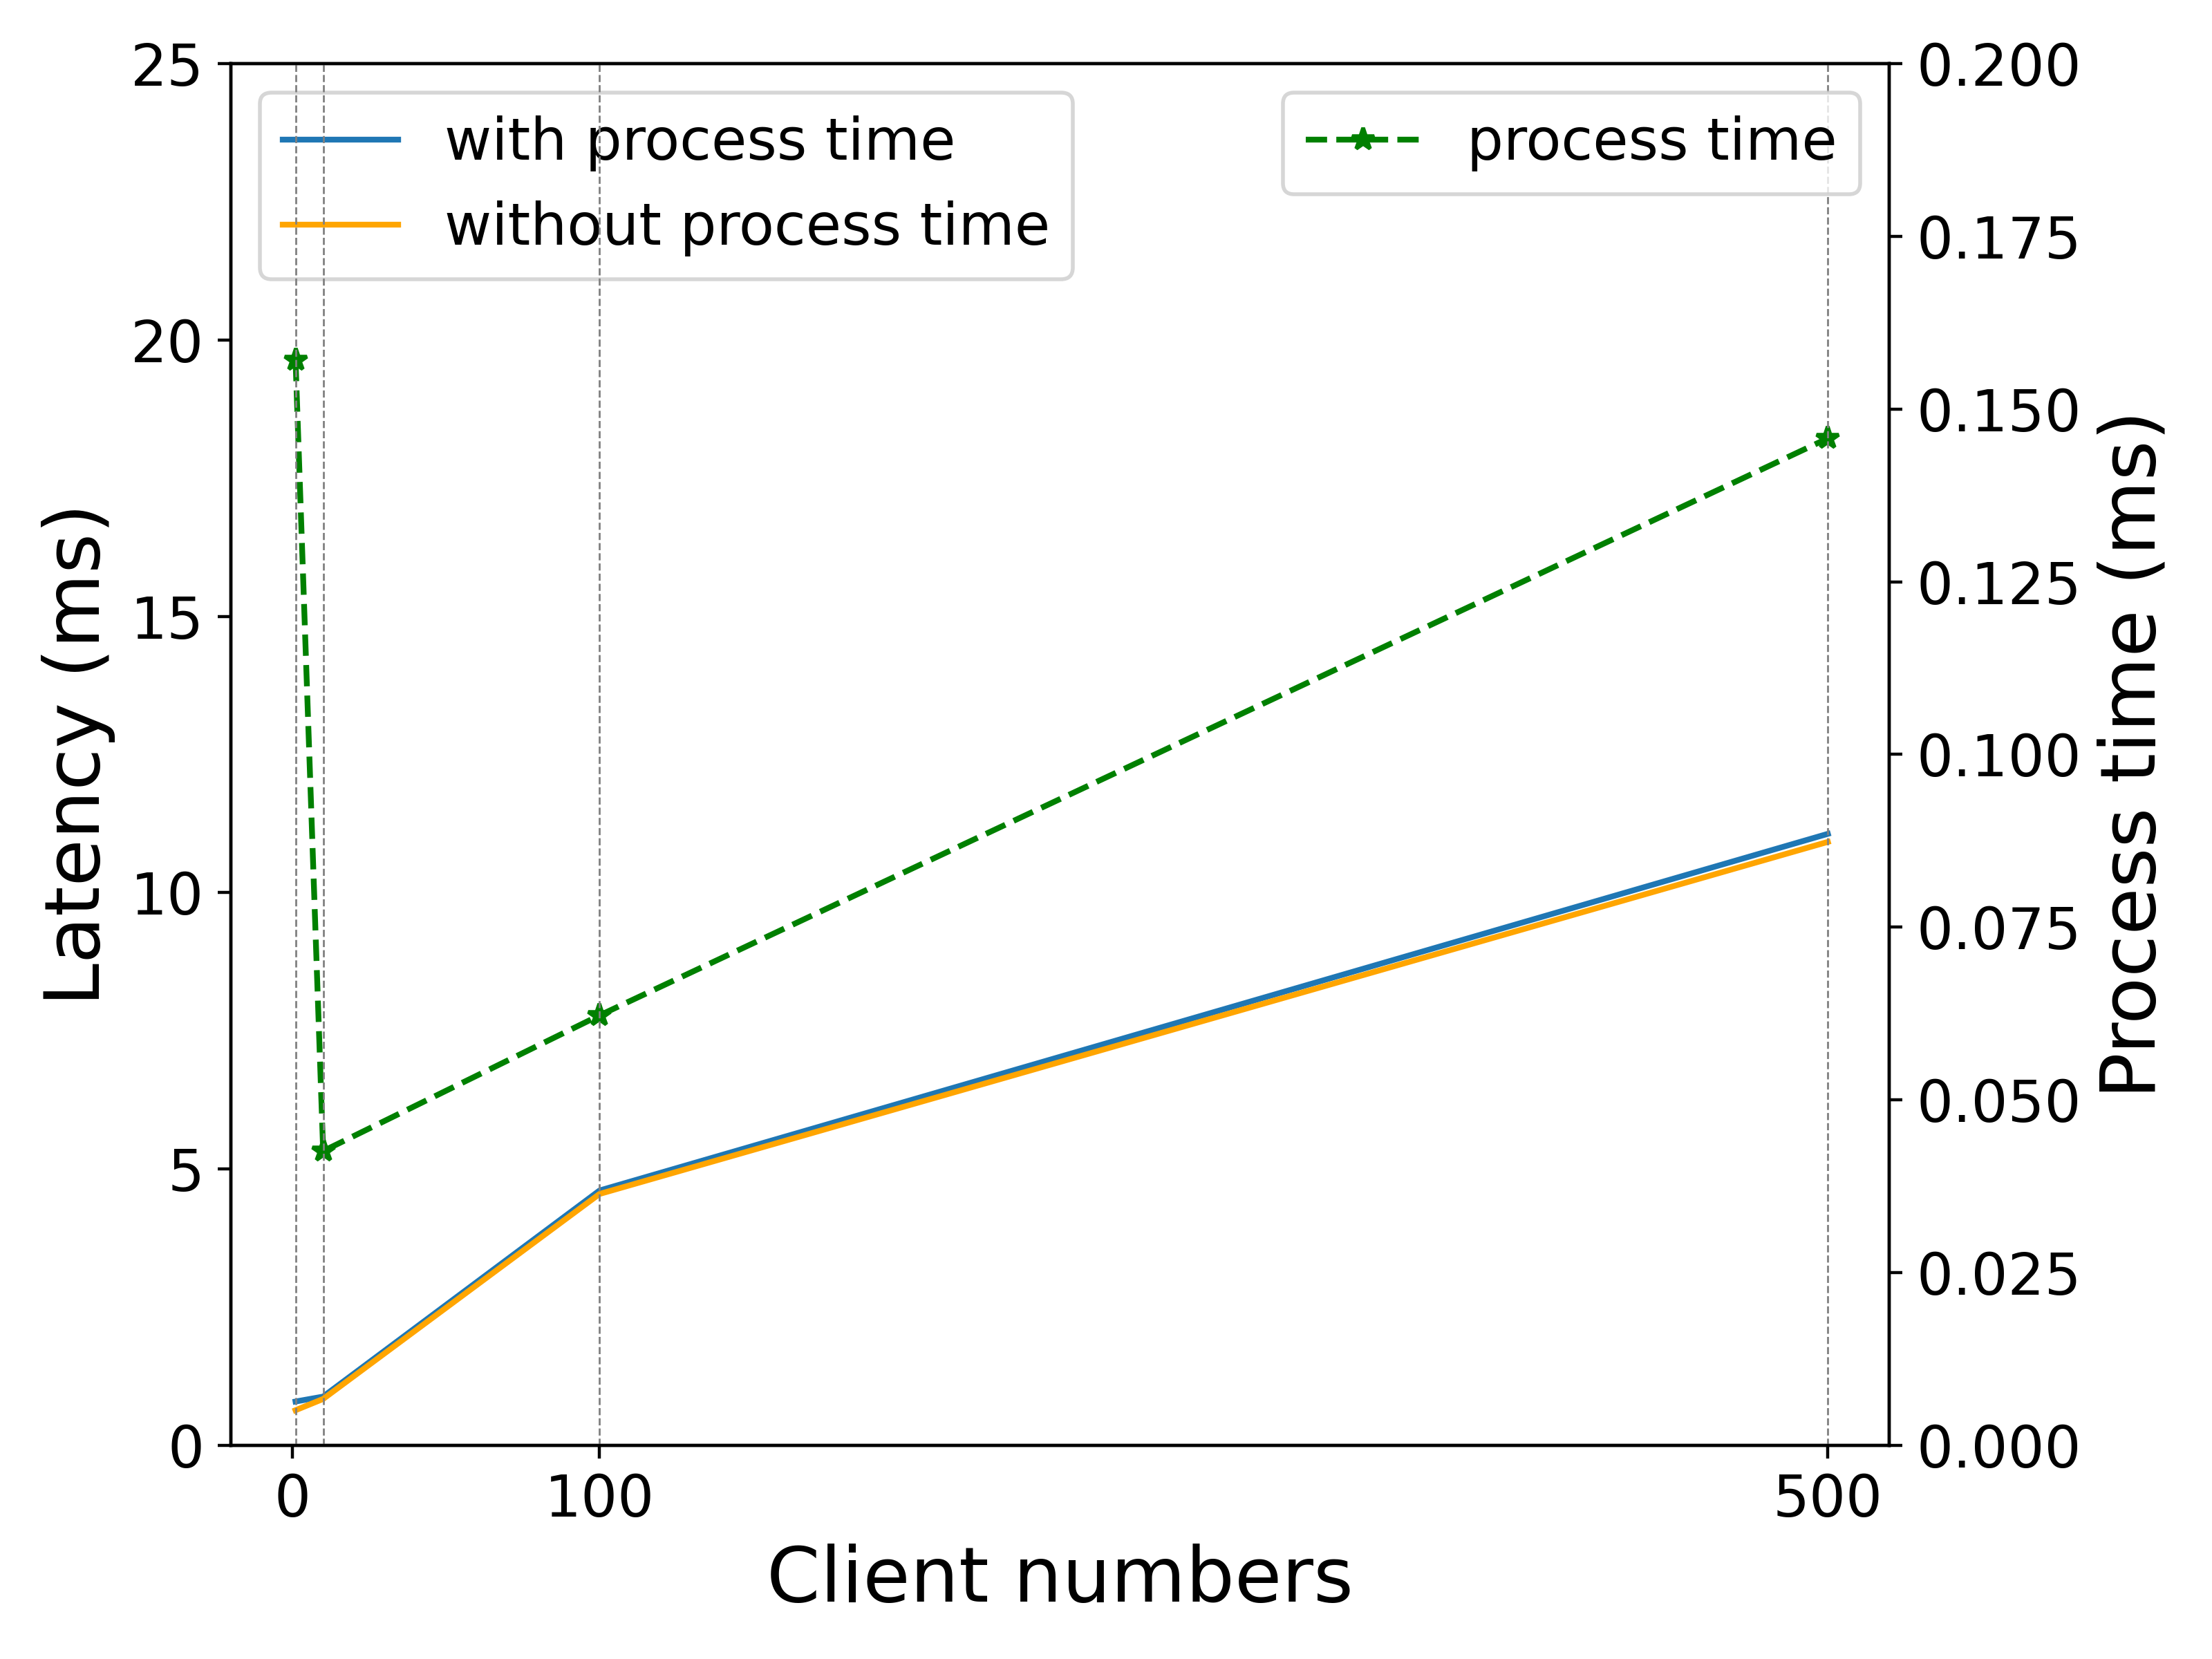
\includegraphics[width=\textwidth]{figures/tests/proportional_tests/Average_string_messages_sending_time_of_100_tests_of_diff_client_numbers.png}\hfill 
        \caption{} \label{fig: proportional-clients-a}
    \end{subfigure}
    \begin{subfigure}[b]{0.49\textwidth}
        \centering
        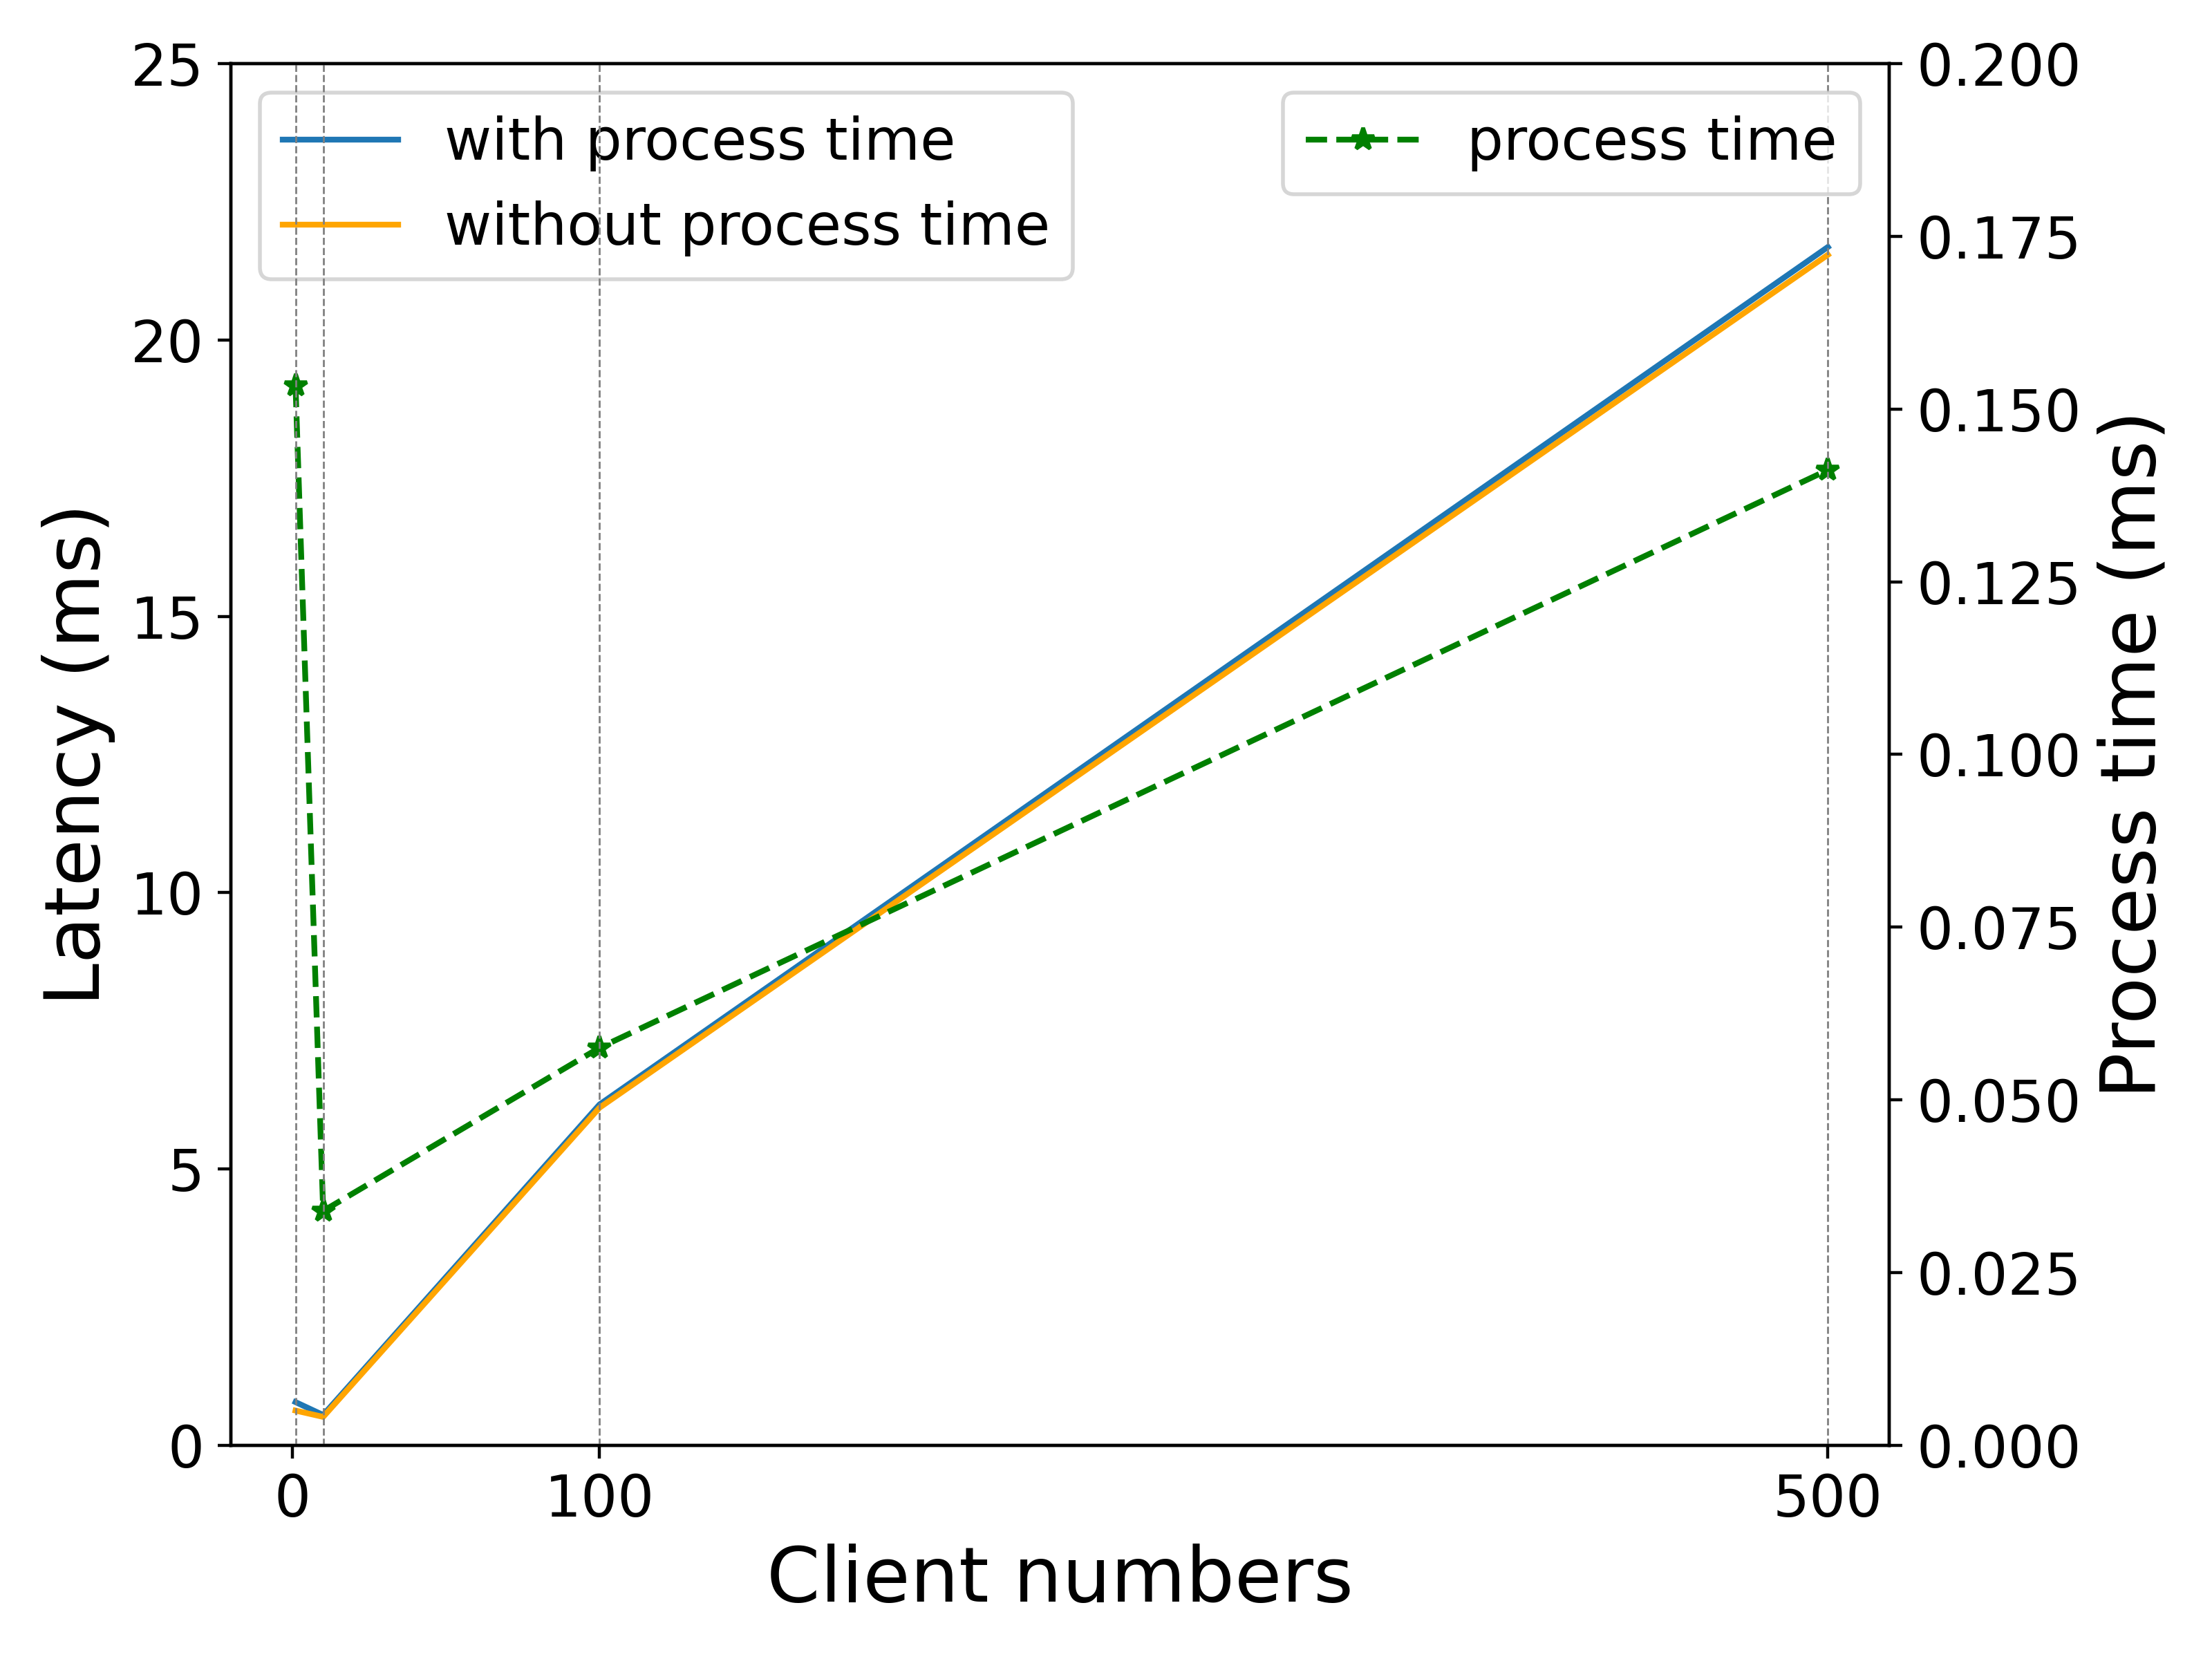
\includegraphics[width=\textwidth]{figures/tests/proportional_tests/Average_string_messages_receiving_time_of_100_tests_of_diff_client_numbers.png}\hfill 
        \caption{} \label{fig: proportional-clients-b}
        \end{subfigure}

    \caption{Average delay of sending a string message 100 times 
    to a clientR from 1, 10, 100 or 500 clients separately. (a) Messages sent forward, 
    and (b) response messages from clientR. 
    \label{fig: proportional-clients}}
\end{figure}


\subsubsection{Increasing server numbers}
Under the same condition where 1000 clients are sending and receiving messages from 
a clientR, the messages will be separated this time to two or three groups, with 
each passing through different servers. Limited by the hardware configuration 
for the external routing solutions according to fig.\ref{fig: NSConceptual}, only 
maximal three servers can be used for the test. However, several assumptions 
can be made based on the results from fig.\ref{fig: proportional-servers}. 


\begin{figure}[htb]
    \centering
    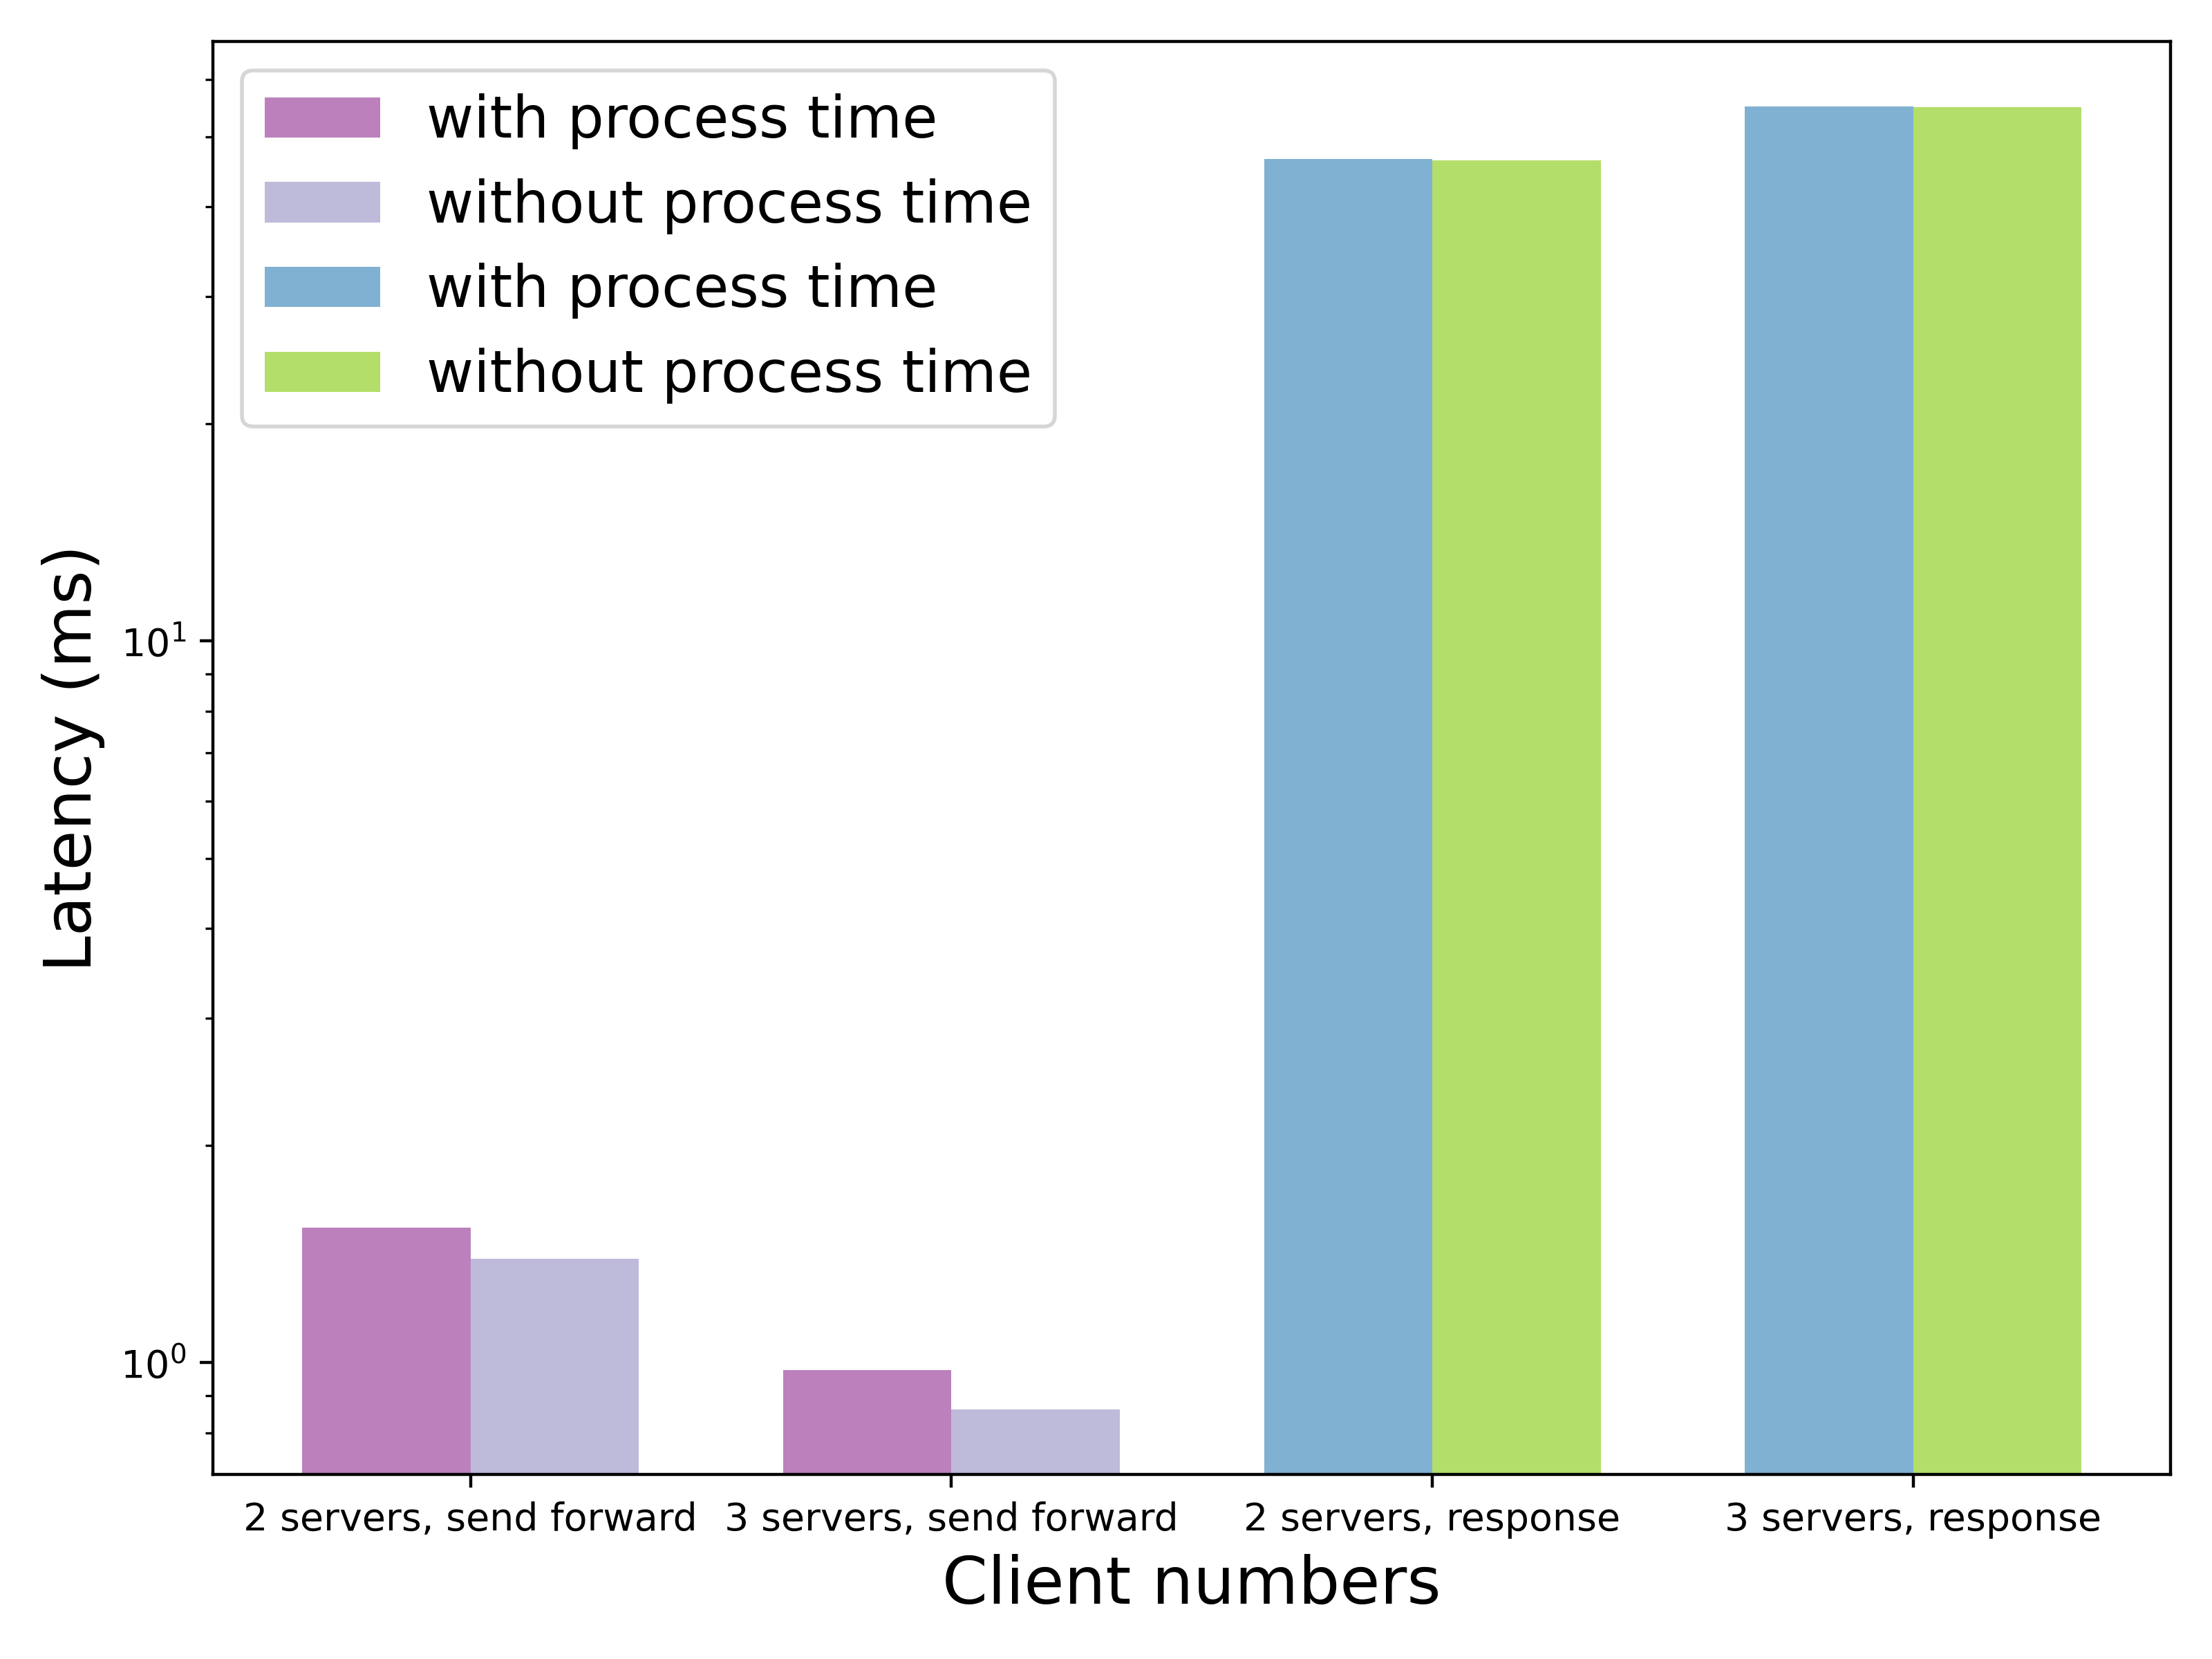
\includegraphics[width=0.8\textwidth]{figures/tests/proportional_tests/Average_string_messages_receiving_time_of_100_tests_diff_server_numbers.png}\hfill 
    \caption{Average delay of sending a string message 100 times 
    to a clientR from 1000 clients through 2 or 3 servers separately. 
    \label{fig: proportional-servers}}
\end{figure}

The latency reduction with an additional server according to 
fig.\ref{fig: proportional-servers} proves that, by introducing more servers 
to the system, the limited productive resources should be better utilized 
for frequent clients interactions. However, not as expected, the latency of 
response messages from clientR is much larger in fig.\ref{fig: proportional-servers},
which may also result from the CPU consumption. Since the send and receive 
processes in websocket are operated separately, and because of the high 
occupation of the CPU power when more than one server are running in the same 
device, the loads between each process might be unbalanced and added up by the 
increment of servers. 


\subsubsection{Increasing string message length}\label{chap: Result-Internal-string}
Another important test should be done to verify the influence of packet size (i.e., 
message length) to the system performance, according to the formula of packet 
transmission time: 
\begin{equation}
    Transmission $ $ delay = Packet $ $ size/Bandwidth
\end{equation}

If the bandwidth is determined, the transmission time with an increasing packet 
size should be linear. In the fig.\ref{fig: proportional-stringsize}, comparisons 
between different string message lengths varied from 1KB to 10MB are examined. 
The linear dependency of latency and string size in both forward 
(fig.\ref{fig: proportional-stringsize-a}) and return message (fig.\ref{fig: proportional-stringsize-b}) 
has verified the transmission time formula. It is also noticeable that the server 
process time increases by the rising message byte number. In real world scenarios, 
a large string message should be chunked into smaller pieces for communication, 
which will significantly reduce the process time consumption. For the purpose of system limit 
inspection, a string with the size up to 100MB is also tested and resulting in 
system timeout error, which already exceeds the server maximal 
processing capacity. 


\begin{figure}[htb]
    \begin{subfigure}{0.49\textwidth}
        \centering
        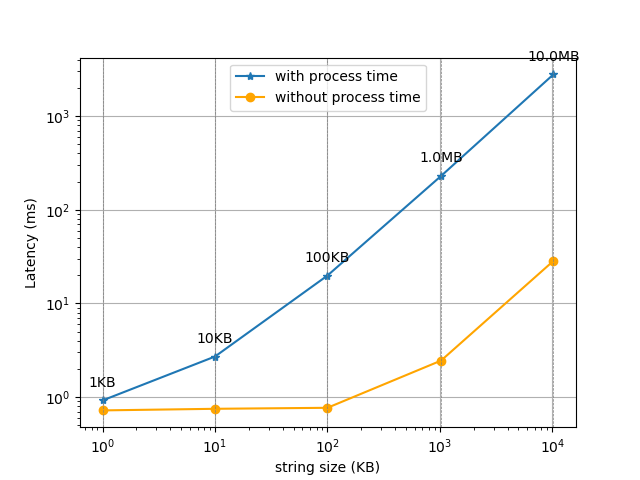
\includegraphics[width=\textwidth]{figures/tests/proportional_tests/log_Average_string_messages_sending_time_of_100_tests_1KB_to_10MB.png}
        \caption{} \label{fig: proportional-stringsize-c}
    \end{subfigure}
    \begin{subfigure}{0.49\textwidth}
        \centering
        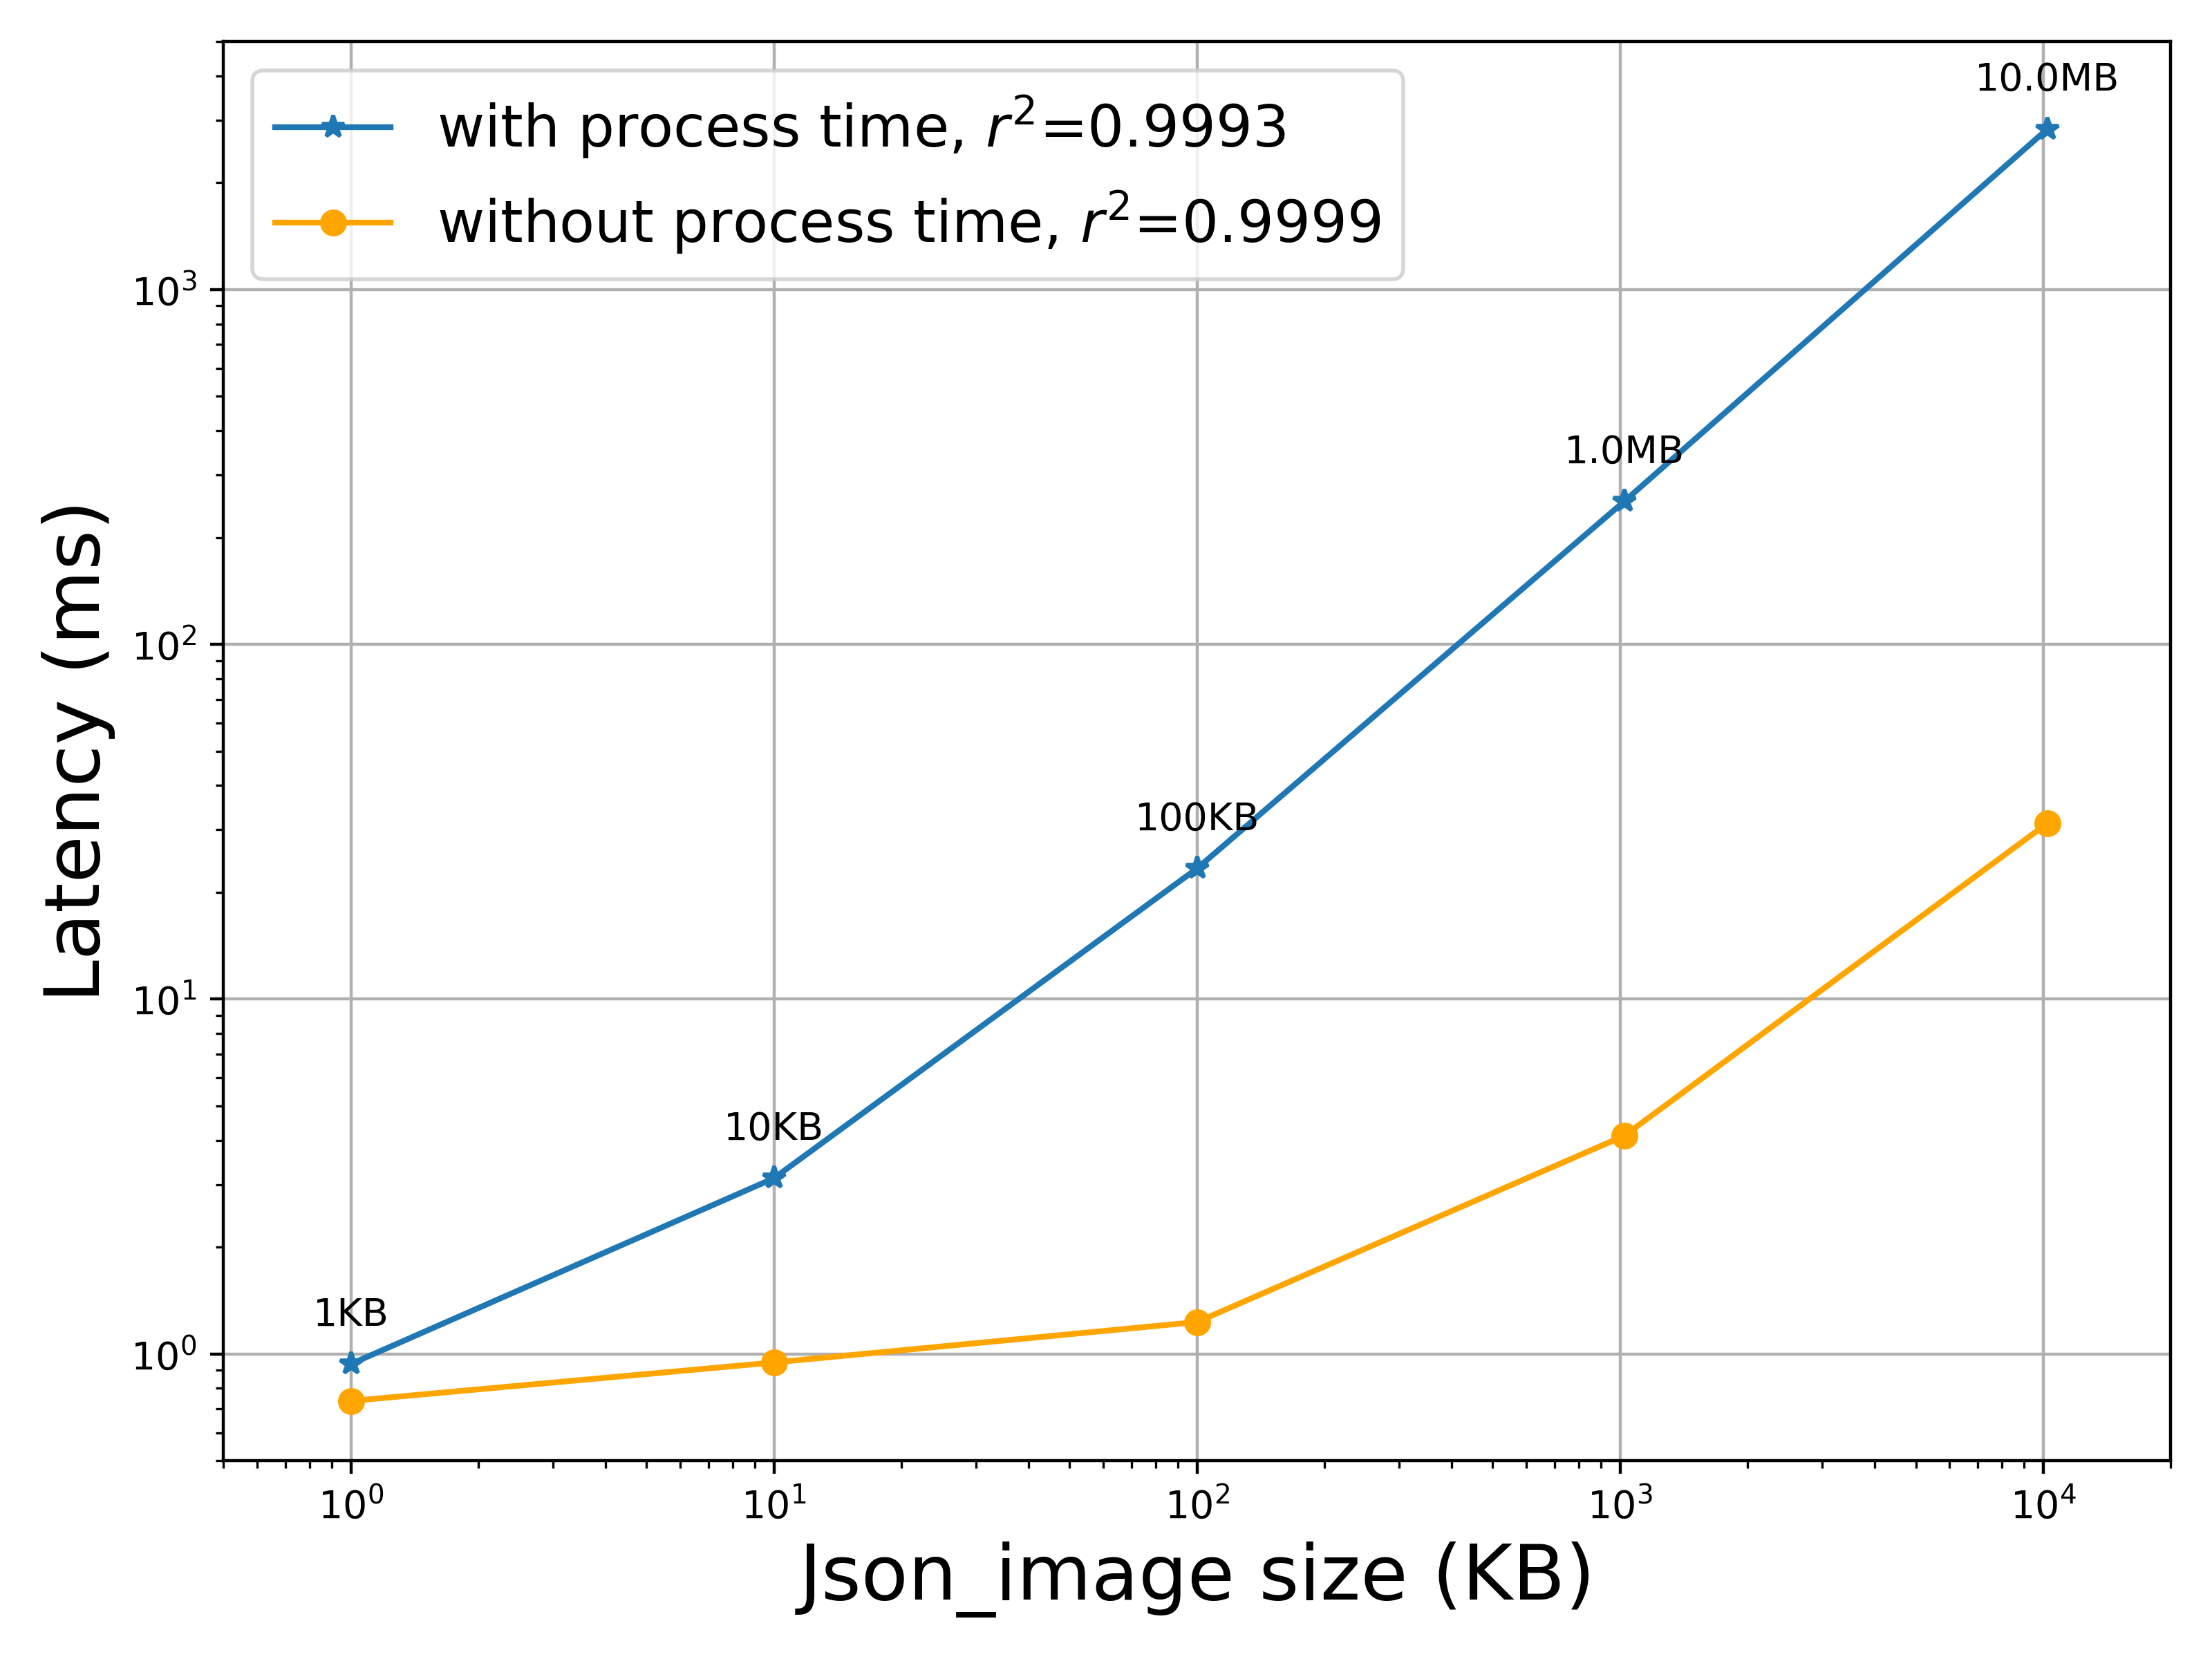
\includegraphics[width=\textwidth]{figures/tests/proportional_tests/log_Average_string_messages_receiving_time_of_100_tests_1KB_to_10MB.png}
        \caption{} \label{fig: proportional-stringsize-d}
    \end{subfigure}

    \begin{subfigure}{0.49\textwidth}
        \centering
        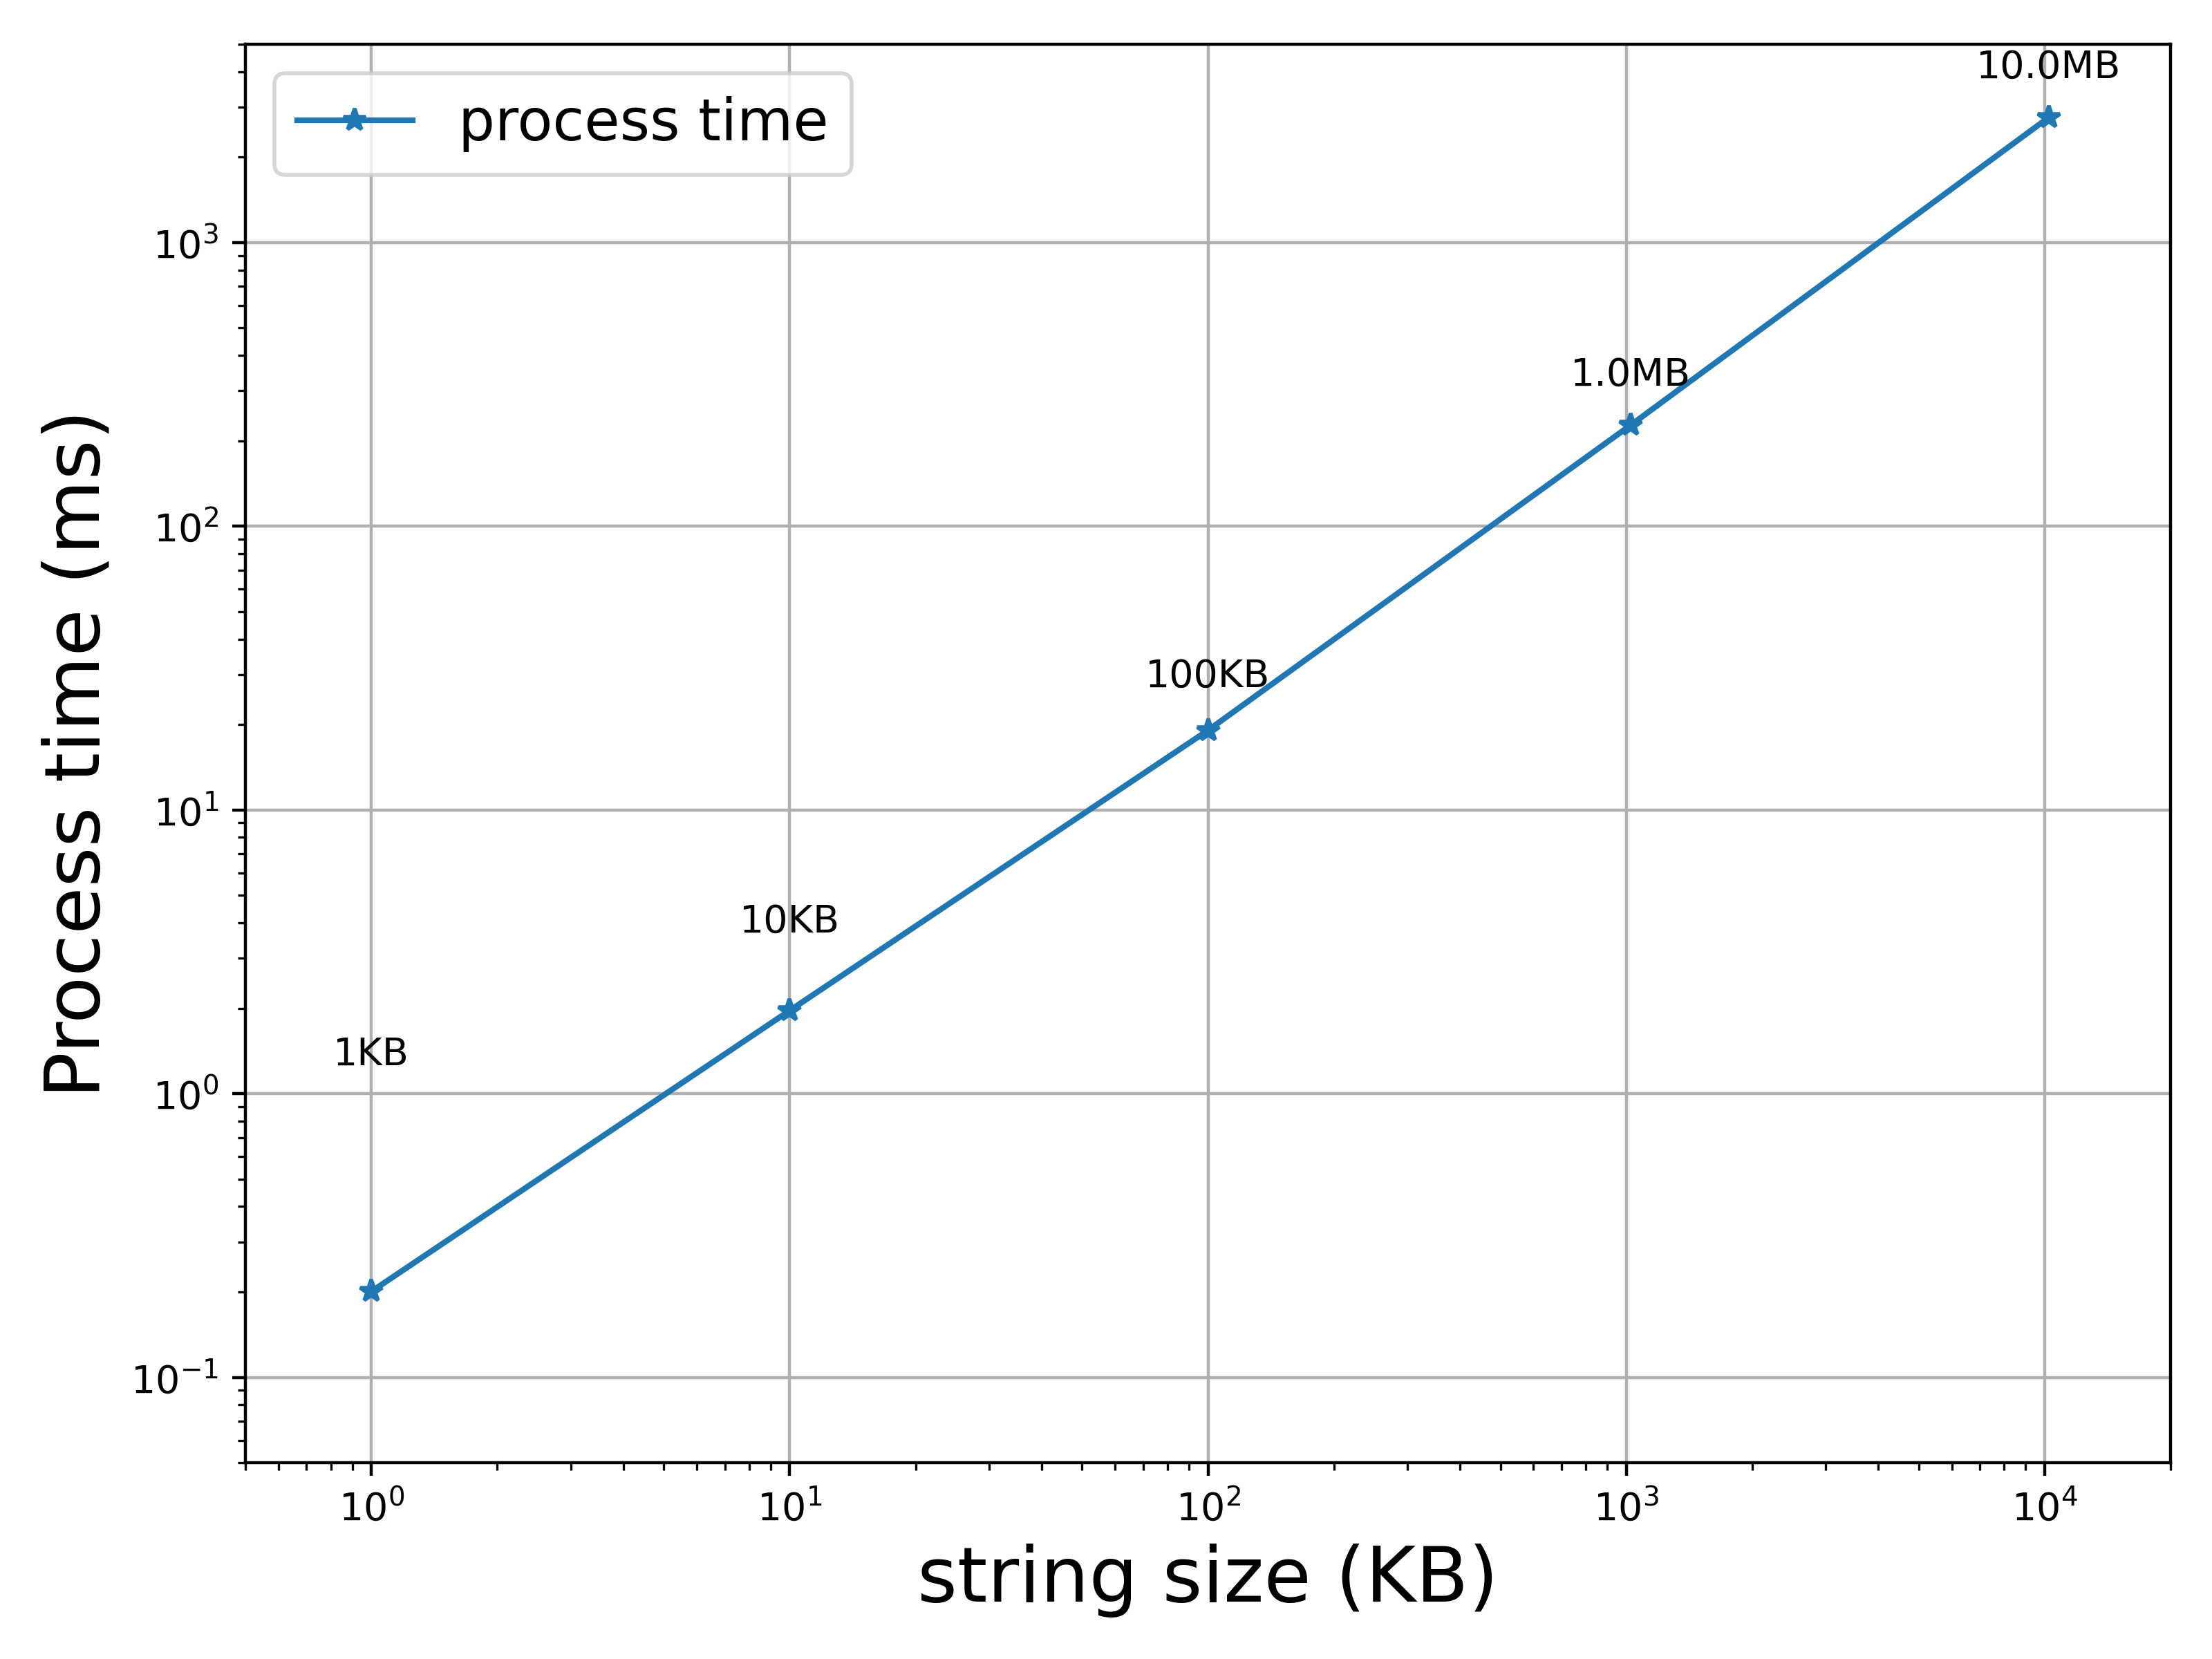
\includegraphics[width=\textwidth]{figures/tests/proportional_tests/Average_string_messages_sending_time_of_100_tests_1KB_to_10MB.png}
        \caption{} \label{fig: proportional-stringsize-a}
    \end{subfigure}
    \begin{subfigure}{0.49\textwidth}
        \centering
        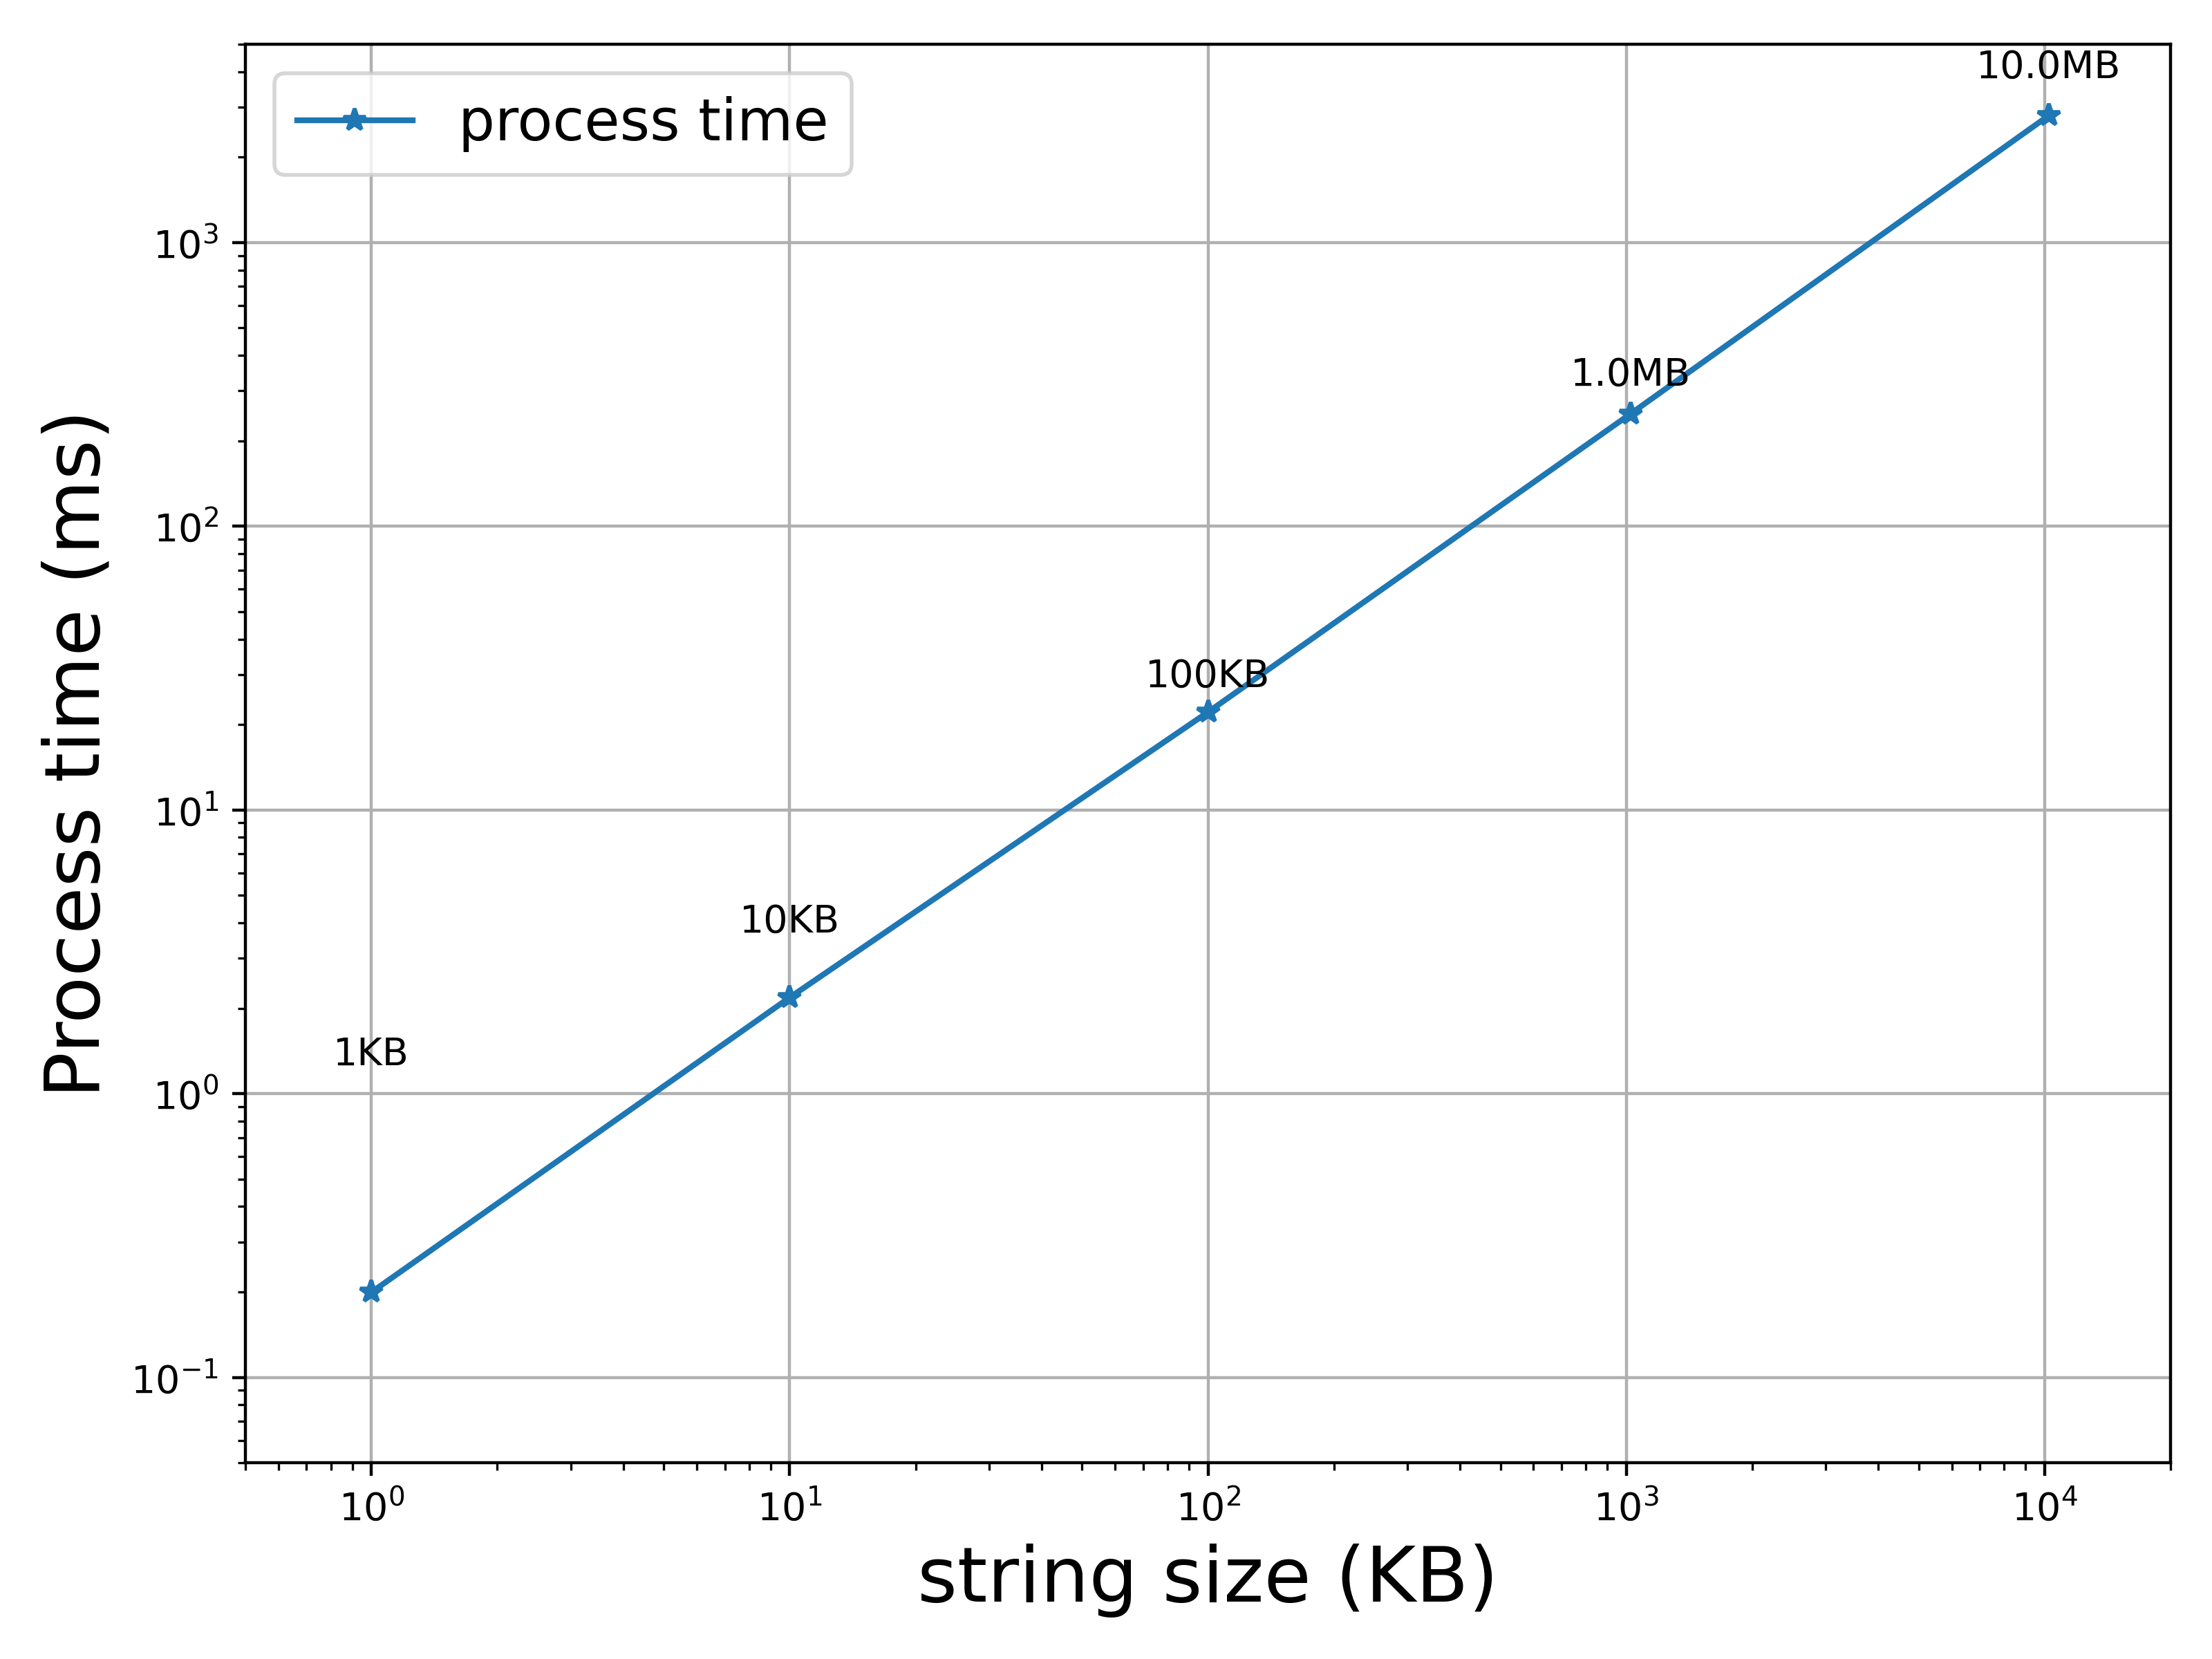
\includegraphics[width=\textwidth]{figures/tests/proportional_tests/Average_string_messages_receiving_time_of_100_tests_1KB_to_10MB.png} 
        \caption{} \label{fig: proportional-stringsize-b}
    \end{subfigure} 

    \caption{Average delay of sending and receiving a string message varied from 1KB 
    to 10MB for 100 times between 2 clients. (\subref{fig: proportional-stringsize-c}) Messages clientS sent forward, 
    (\subref{fig: proportional-stringsize-d}) response messages from clientR, 
    (\subref{fig: proportional-stringsize-a}) process time of massages sent forward 
    and (\subref{fig: proportional-stringsize-b}) process time of massages respond. 
    \label{fig: proportional-stringsize}}
\end{figure}

\subsubsection{Increasing image message length}
In addition to string, images are also frequently tranported between different agents. 
However, unlike most string messages, image size could be significantly larger 
and even up to over 100MB (raw images). Moreover, the agents ID or message priority 
information should also be included in the message. Therefore, the image should 
be first jsonified with necessary information and then sent to the server. 
The tests for images are done similar to the string message, with an image size 
varies from 1KB to 100MB. 


In fig.\ref{fig: proportional-imagesize-a} and \ref{fig: proportional-imagesize-b} 
again shows the linear dependency of latency and jsonified image size. 
Although the image test results in a 
transmisson time from 1KB to 10MB message length similar to string test, 
there is a huge difference in terms of process time between both. By comparing the 
fig.\ref{fig: proportional-stringsize-c} with \ref{fig: proportional-imagesize-c} 
and fig.\ref{fig: proportional-stringsize-d} with \ref{fig: proportional-imagesize-d}, 
the server process time of string messages is much higher than that for the 
image message. Meanwhile, due to the additional overhead of json format, the network 
delay of string messages is relative smaller than image messages. 


A possible reason for the larger process time for string is that, a string message 
received by server must be processed twice: splitting the message to extract the client 
ID and recombining it for further transport. Meanwhile a jsonified image will only be 
processed once to extract the client information and the original json file will be 
futher transported directly.     
\begin{figure}[htb]
        \centering
    \begin{subfigure}{0.49\textwidth}
        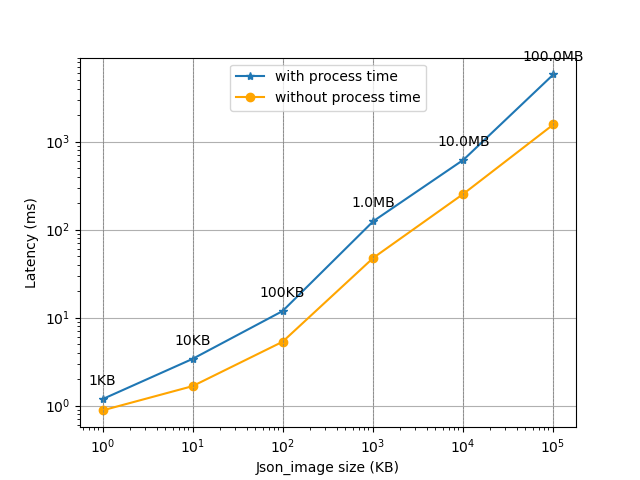
\includegraphics[width=\textwidth]{figures/tests/proportional_tests/log_Average_json_image_messages_sending_time_of_100_tests_1KB_to_100MB.png}\hfill 
        \caption{} \label{fig: proportional-imagesize-c}
    \end{subfigure}
    \begin{subfigure}{0.49\textwidth}
        \centering
        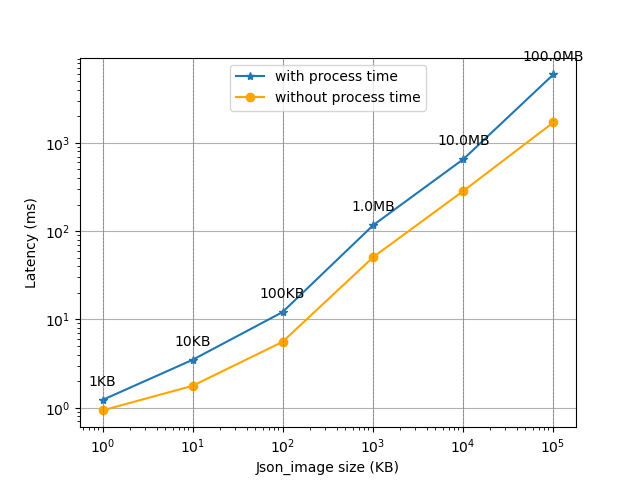
\includegraphics[width=\textwidth]{figures/tests/proportional_tests/log_Average_json_image_messages_receiving_time_of_100_tests_1KB_to_100MB.png}\hfill 
        \caption{} \label{fig: proportional-imagesize-d}
    \end{subfigure}
    \begin{subfigure}{0.49\textwidth}
        \centering
        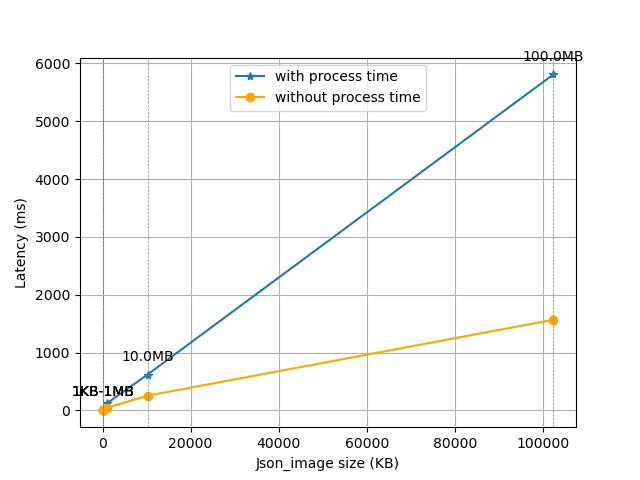
\includegraphics[width=\textwidth]{figures/tests/proportional_tests/Average_json_image_messages_sending_time_of_100_tests_1KB_to_100MB.png}\hfill 
        \caption{} \label{fig: proportional-imagesize-a}
    \end{subfigure}
    \begin{subfigure}{0.49\textwidth}
        \centering
        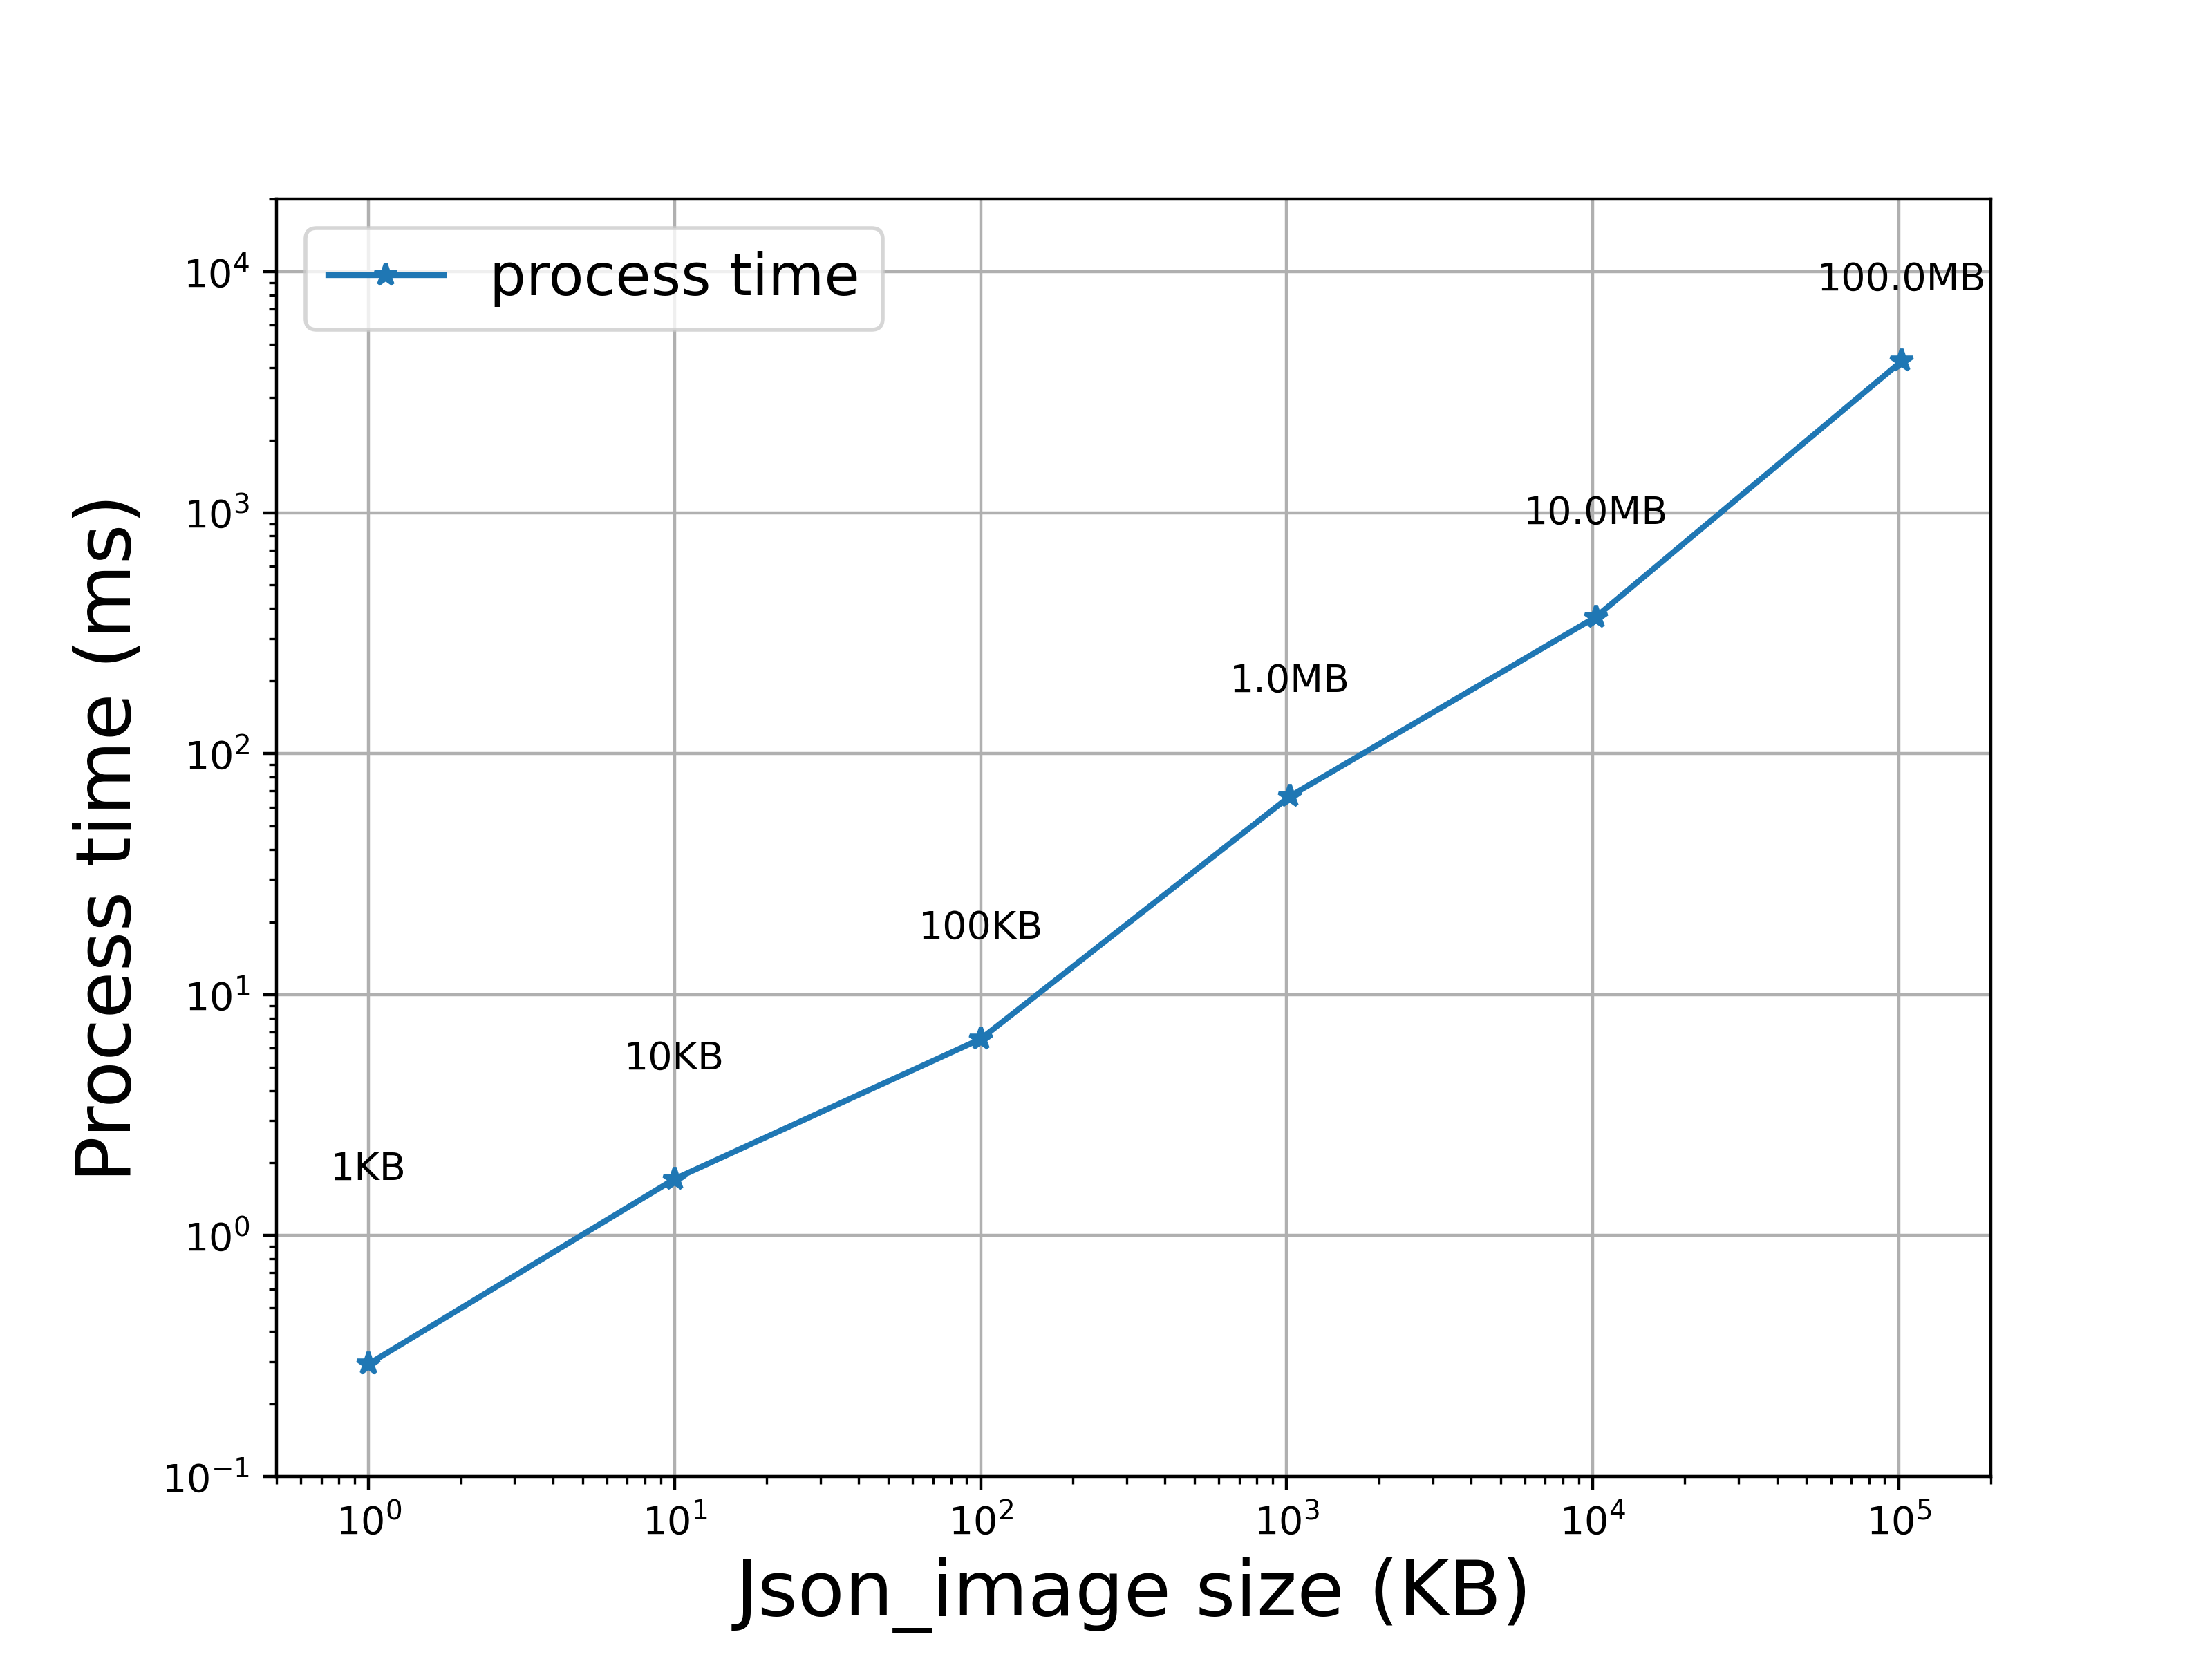
\includegraphics[width=\textwidth]{figures/tests/proportional_tests/Average_json_image_messages_receiving_time_of_100_tests_1KB_to_100MB.png}\hfill 
        \caption{} \label{fig: proportional-imagesize-b}
    \end{subfigure}

    \caption{Average delay of sending and receiving a jsonified image message varied from 1KB 
    to 100MB for 100 times between 2 clients. (\subref{fig: proportional-imagesize-c}) 
    Messages clientS sent forward in log form, 
    (\subref{fig: proportional-imagesize-d}) response messages from clientR in log form, 
    (\subref{fig: proportional-imagesize-a}) process time of messages sent forward  
    and (\subref{fig: proportional-imagesize-b}) process time of response messages from clientR. 
    \label{fig: proportional-imagesize}}
\end{figure}


\subsection{Test results of WebSocket and \gls{http}} \label{chap: Result-RestFUL_WS}
After testing the performance of the WebSocket based communication system, 
it will be interesting to see whether the other application layer protocols with 
different message transport mechanism will have a similar or completely different 
performance under the same conditions. As demonstrated from the 
fig.\ref{fig: MsgConceptual}, \gls{http} is designed for message 
transfer in both directions, and therefore more comparable with WebSocket among the others. 
As a result, a \gls{http} based interface RESTful API is designed under the similar architecture 
as WebSocket and tested under the same condition of the WebSocket string test in 
section \ref{chap: Result-Internal-string}. By comparing 
fig.\ref{fig: proportional-stringsize} with fig.\ref{fig: proportional-rest-stringsize}, 
it is obvious that the process time of string messages is higher and 
grows faster in a WebSocket server than RESTful API server. The difference may 
results in the prioritization and data processing mechanisms in WebSocket server, 
while RESTful API server is only designed with basic message POST and GET 
mechanism. However, the data transmission time between both is more comparable. 
First of all, both of them reflect the fit of the model with the coefficient 
of determination closes to one, which is namely: 


    \begin{align}
        R^{2} &= 1-\frac{RSS}{TSS}\\
        \text{Where} \nonumber\\
        RSS & = \text{sum of squared residuals} \nonumber\\
        TSS & = \text{total sum of squares}\nonumber
    \end{align}

meaning that the model fits the data well.





Secondly, the transmission time of both is similar 
with respect to the same string message length (RESTful has slightly higher latency), 
with a difference of 0.01ms to few milliseconds, which grows over 
message size.   

Therefore, WebSocket is proven to be more appropriate for real time message 
transfer, which is essential for an agent based system.


\begin{figure}[htb]
    \begin{subfigure}[b]{0.49\textwidth}
        \centering
        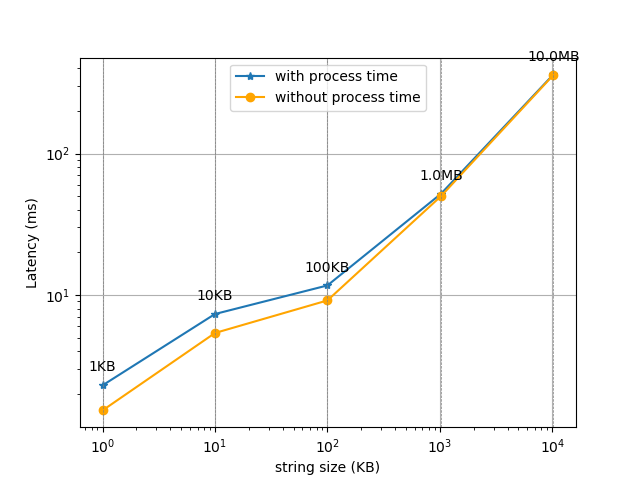
\includegraphics[width=\textwidth]{figures/tests/proportional_tests/Rest_log_Average_string_messages_sending_time_of_100_tests.png}\hfill 
        \caption{} \label{fig: proportional-rest-stringsize-c}
    \end{subfigure}
    \begin{subfigure}[b]{0.49\textwidth}
        \centering
        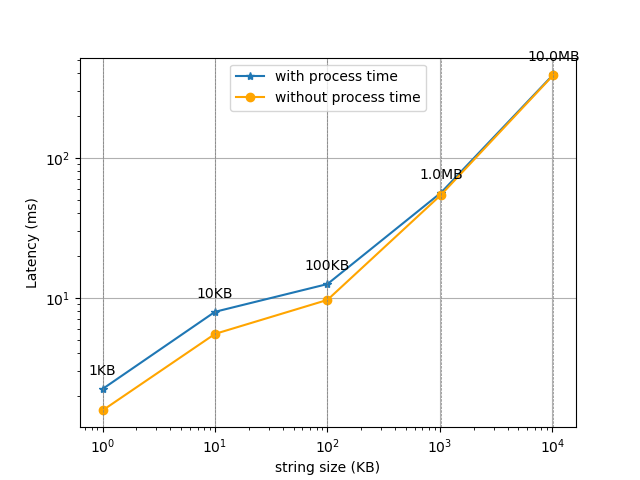
\includegraphics[width=\textwidth]{figures/tests/proportional_tests/Rest_log_Average_string_messages_receiving_time_of_100_tests.png}\hfill 
        \caption{} \label{fig: proportional-rest-stringsize-d}
    \end{subfigure}

    \begin{subfigure}[b]{0.49\textwidth}
        \centering
        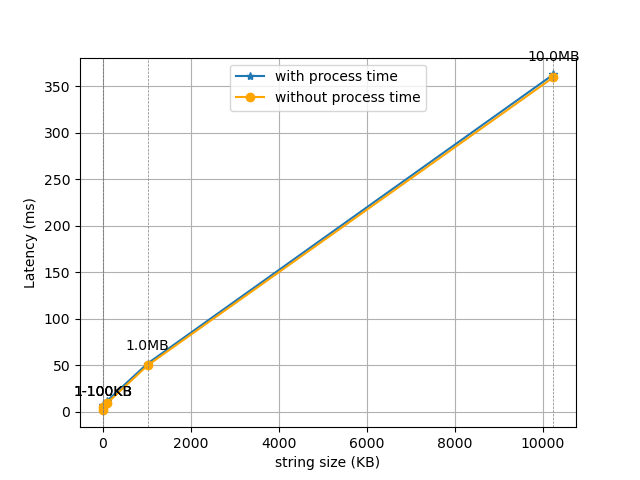
\includegraphics[width=\textwidth]{figures/tests/proportional_tests/Rest_Average_string_messages_sending_time_of_100_tests.png}\hfill 
        \caption{} \label{fig: proportional-rest-stringsize-a}
    \end{subfigure}
    \begin{subfigure}[b]{0.49\textwidth}
        \centering
        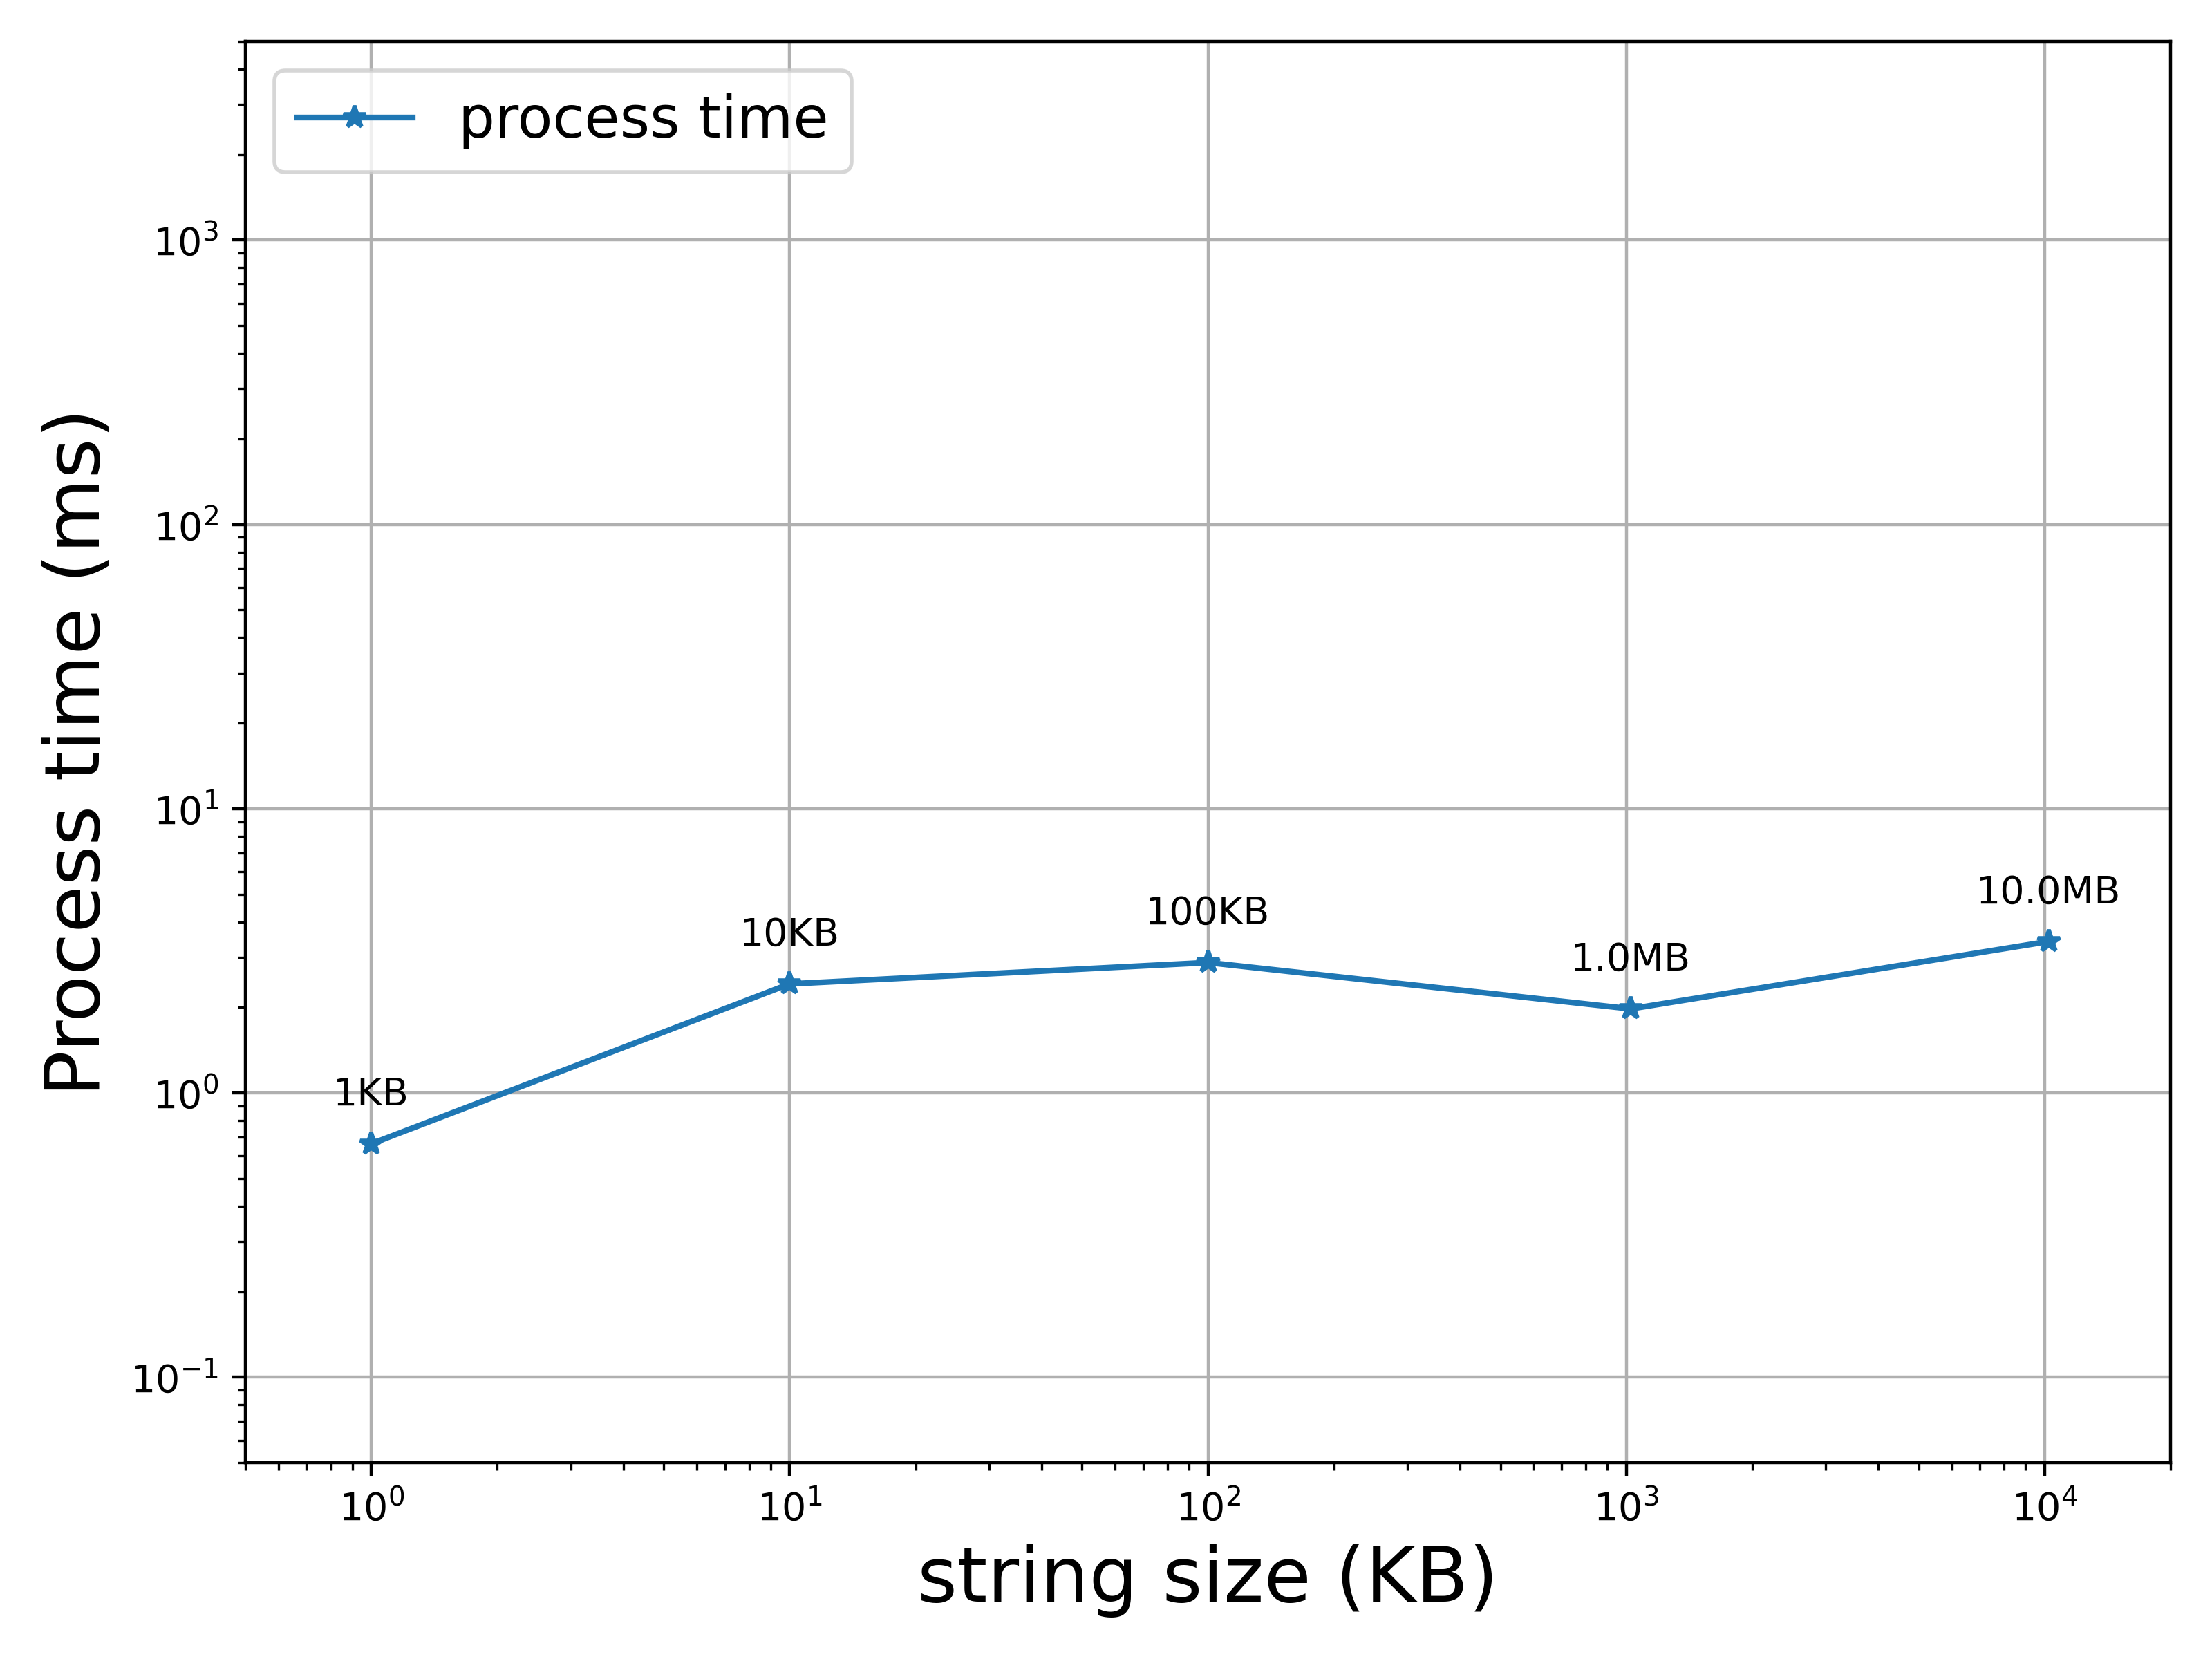
\includegraphics[width=\textwidth]{figures/tests/proportional_tests/Rest_Average_string_messages_receiving_time_of_100_tests.png}\hfill 
        \caption{} \label{fig: proportional-rest-stringsize-b}
    \end{subfigure}
    
    \caption{RESTful API: Average delay of sending and receiving a string message varied from 1KB 
    to 10MB for 100 times between 2 clients. (\subref{fig: proportional-rest-stringsize-c}) 
    Messages clientS sent forward, 
    (\subref{fig: proportional-rest-stringsize-d}) response messages from clientR, 
    (\subref{fig: proportional-rest-stringsize-a}) process time of messages sent forward 
    and (\subref{fig: proportional-rest-stringsize-b}) process time of messages respond. 
    \label{fig: proportional-rest-stringsize}}
\end{figure}





\subsection{Test results of message prioritization of a WebSocket server in various 
performance testing} \label{chap: Result-priority}
Apart from the consideration of speed, robustness, reliability and application size in an agent 
communication system, the server which serves as a \gls{ca} should have addtional 
functionalities rather than pure message transport. As listed in tab.\ref{tab:designPatterns}, 
the \gls{ca} should focus on the design of a communication interface, which should be able to 
process various messages with different data types (e.g., jsonified images), handle a large 
number of agents connections and prioritize the incoming messages. In the following sections, 
the performance of server handling message prioritization will be tested and further discussed.  

\subsubsection{Measurgin method}
In order to verify the prioritization mechanism of the server, a delay of 1s should be added to the 
non-prioritized message processing. In the test, two kinds of messages are sent conccurently to the server, 
the normal and the critical messages. If more than one message with different priority levels 
enter the server simultaneously, the critical messages should be processed first. The add up of 
delay also reflects the real world scenarios: if a critical message representing an emergent stop 
or a task with higher priority in production comes in, every other processe in the server 
should wait until the critical message is sent. 

\subsubsection{String message priority test}
The first string priority test is done for 10 clients. The following fig.\ref{fig: priority-10clients-a} 
and \ref{fig: priority-10clients-b} shows the mean \gls{rtt} 
that a non-prioritized and prioritized message being sent forward and back separately for 100 times.
In fig.\ref{fig: priority-10clients-a}, the mean \gls{rtt} for client1 to client10 in both directions 
varies from 0.63ms to 1.09ms, 
which fullfills the near real time requirement(quote) for production process. 
The fig.\ref{fig: priority-10clients-b} on the other hand, 
presents the timing differences of normal messages as a group and critical messages as control group. 
In the test, all clients deliver normal messages except for client10. That means, whenever a critical 
message from client10 arrives, the server will pause the other processes for 1s and handle the 
critical message immediately. In the test, the mean \gls{rtt} for client10 is less than 1ms. 
In contrast, clients such as client1 through client5 and client9 experience 
significantly higher RTTs, sometimes reaching several hundred milliseconds, which 
has verified the assumption of message prioritization. It is worth mentioning that, due to the concurrent 
nature of the asyncio package in the WebSocket server design, each client will be executed 
one after another, different from parallel processing. That means, some messages may never be paused 
if the clients execution process is not synchronized and coordinated explicitly. 

\begin{sidewaysfigure}[htb]
    \centering
    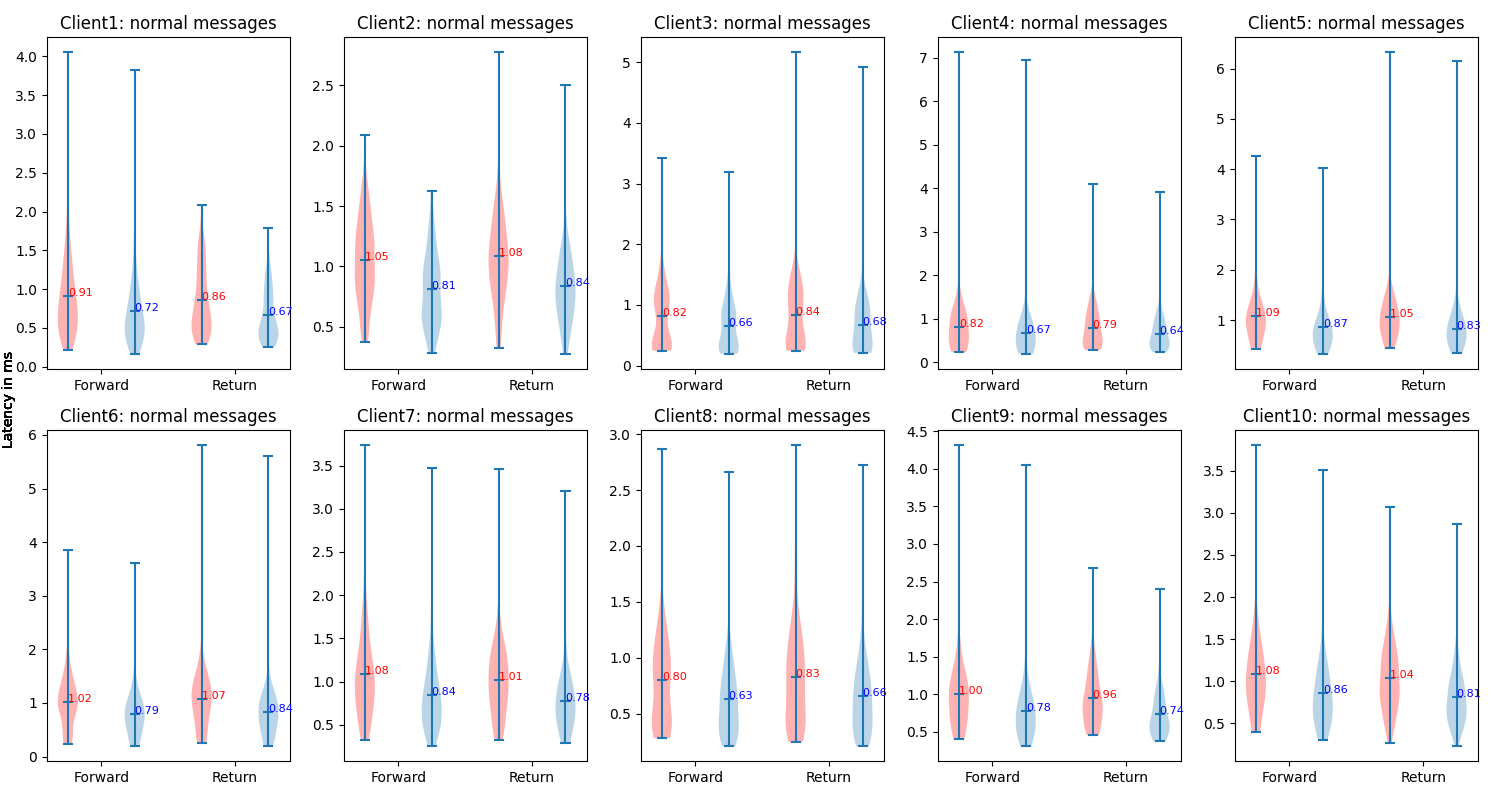
\includegraphics[width=\textheight]{figures/tests/priority_tests/violin_10clients_string_non_priority.png}\hfill 
    \caption{Tests for mean \gls{rtt} of forward and return non-prioritized string messages between 10 clients 
    and clientR for 100 times. The blue violin represents the average data transmission time and the red violin 
    respresent mean \gls{rtt}.} \label{fig: priority-10clients-a}
\end{sidewaysfigure}
\begin{sidewaysfigure}[htb]
    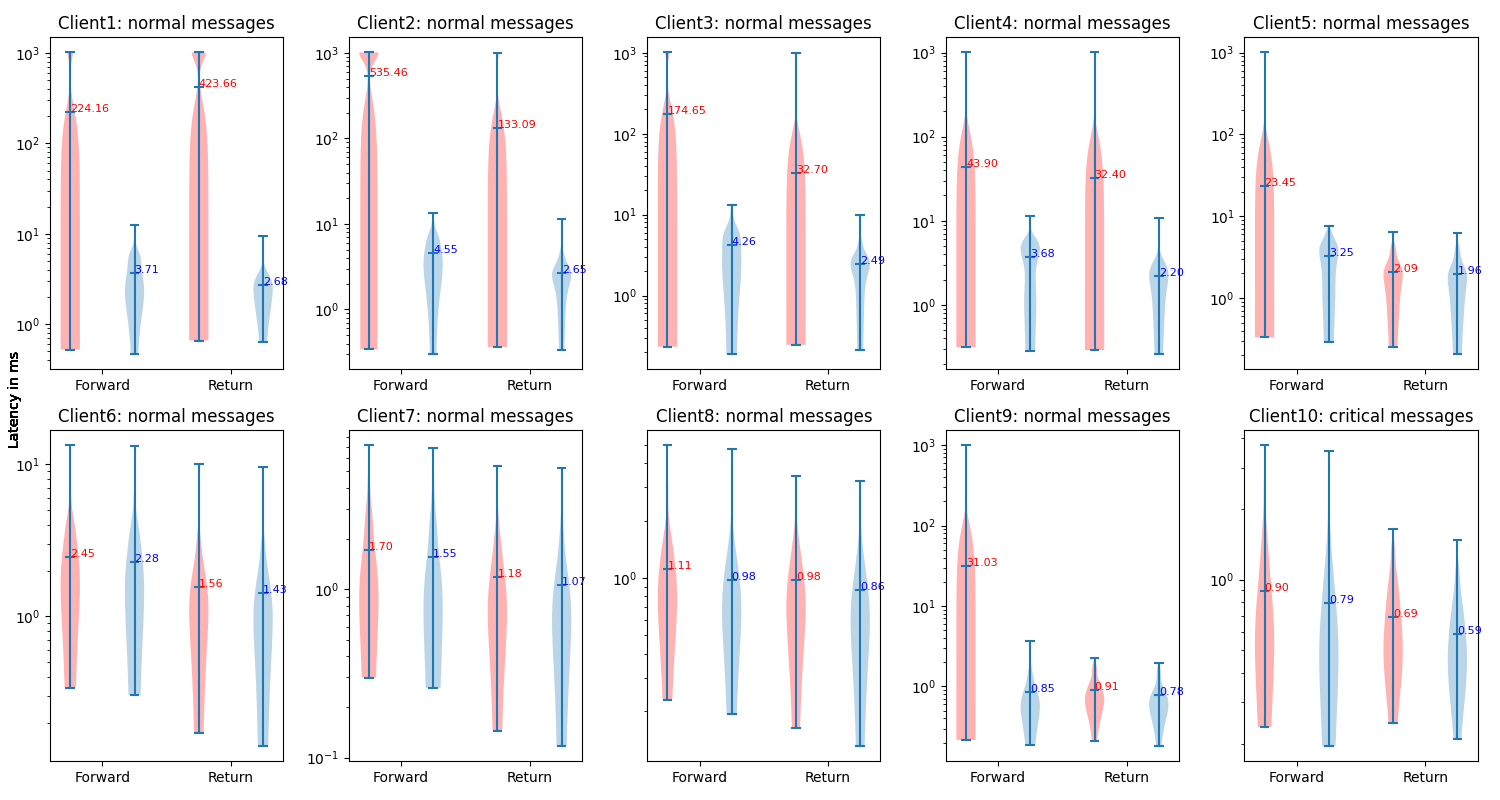
\includegraphics[width=\textheight]{figures/tests/priority_tests/log_violin_10clients_string_priority.png}\hfill 
    \caption{Tests for mean \gls{rtt} of forward and return prioritized string messages between 10 clients 
    and clientR for 100 times. The blue violin represents the average data transmission time and the red violin 
    respresent mean \gls{rtt}.} \label{fig: priority-10clients-b}
\end{sidewaysfigure}



Together with the priority tests for 10 clients, there are similar tests performed in different scales. 
In all these tests, the number of clients varies from 2, 10 to 50. The test results 
of 2 clients can be found in \ref{chap: append-string-priority} fig.\ref{fig: priority-2clients-string}, 
and those for 50 clients in fig.\ref{fig: priority-50clients-string-a} to 
\ref{fig: priority-50clients-string-e}. For the string message priority test with 2 clients, 
it is clear that client1 sends messages with lower priority results in 
a much higher delay than client2 in both directions. As for the test with 50 clients, 
the test result is similar to those in the test for 10 clients. In the test, only the 
last client will send a critical message, while the other 49 clients with a normal message. 
This resulted in some clients being affected by the mechanism and greatly increasing delays, 
while client50 will always have a smallest \gls{rtt}.

\subsubsection{Image message priority test}
The same tests are also done for image message transport. Slightly different 
from string messages, the prioritization jsonified image file (image size: 33.4KB) 
will be performed 
after deserialization. In the image priority test, client1 to client10 will send an 
image to clientR, and receive a string message as response. In actual production,
a confirm string message will be sent back if the image message is successfully received 
by clientR. Therefore, this test can better reflect the time difference between 
different messages types in the actual production process, since mostly the actual 
string length will be much smaller than the image length. As shown in fig.\ref{fig: priority-10clients-c}, 
it proves that either the data transmission time or the server process time of a image message 
will be higher than a string message.


\begin{sidewaysfigure}[htb]
    \centering
    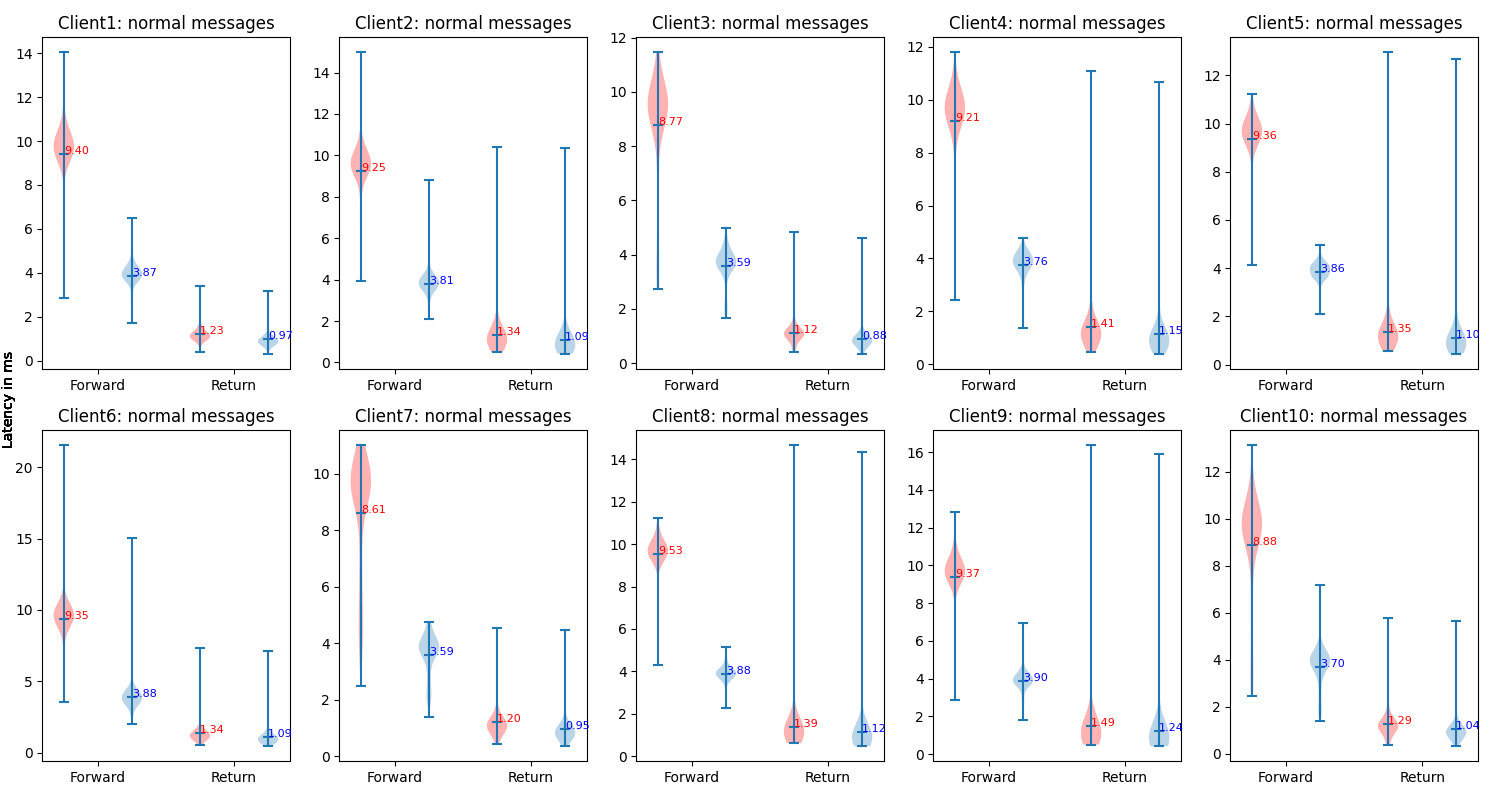
\includegraphics[width=\textheight]{figures/tests/priority_tests/violin_10clients_image_non_priority.png}\hfill 
    \caption{Tests for mean \gls{rtt} of non-prioritized forward image messages and return string messages between 10 clients 
    and clientR for 100 times. The blue violin represents the average data transmission time and the red violin 
    respresent mean \gls{rtt}.} \label{fig: priority-10clients-c}
\end{sidewaysfigure}


Another test (fig.\ref{fig: priority-10clients-d}) should be similar to the string message priority test (fig.\ref{fig: priority-10clients-b}), 
with 2, 10 and 50 clients sending images and receiving string messages as response 
from clientR. 
All client1 to client9 send a normal image message and meanwhile 
client10 sends a critical one to clientR. 
In the test, all image messages and only a part of the response string messages 
being sent trigger the prioritization mechanism.  In this, the latency for 
the prioritized string messages is very similar to previous test results
The reason might be that the larger the file size, the longer the transfer 
and processing time will required. The larger message length of images 
results in more data bytes 
that needs to be processed simultaneously, which involves the a higher number of 
message queuing and message prioritization in server. The same conclusion can be 
also made for the tests for 2 and 50 clients in \ref{chap: append-image-priority} fig.\ref{fig: priority-2clients-image} 
to \ref{fig: priority-50clients-image-e}.


\begin{sidewaysfigure}[htb]
    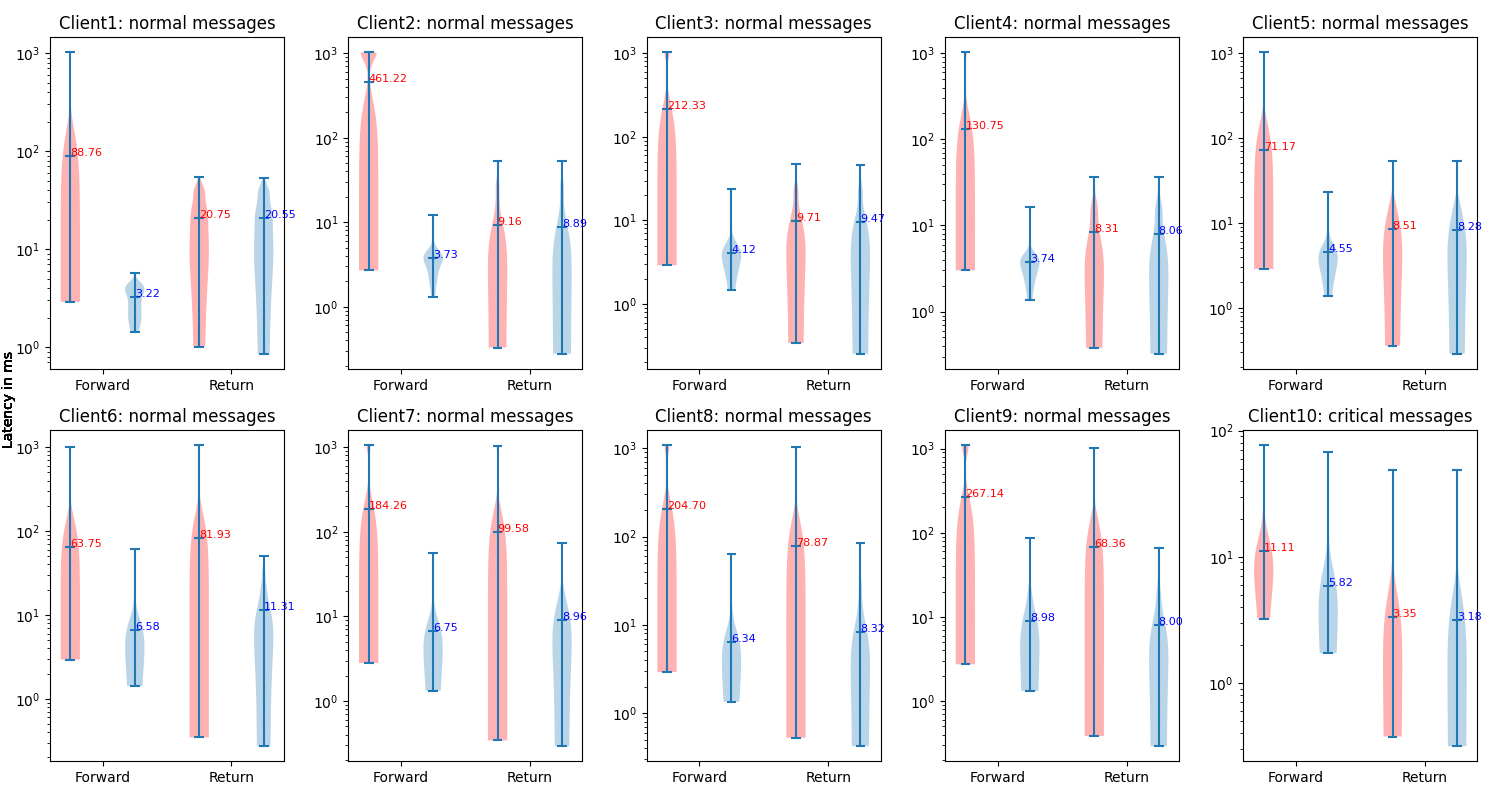
\includegraphics[width=\textheight]{figures/tests/priority_tests/log_violin_10clients_image_priority.png}\hfill 
    \caption{Tests for mean \gls{rtt} of prioritized forward image messages and return string messages between 10 clients 
    and clientR for 100 times. The blue violin represents the average data transmission time and the red violin 
    respresent mean \gls{rtt}.} \label{fig: priority-10clients-d}
\end{sidewaysfigure}


\subsection{Diagrams of WebSocket based \gls{mas} architecture under two use cases and test 
test results of BMW use case}\label{chap: Result-Internal-Usecase}
As listed earlier in form of pseudocode in section \ref{chap: Meth-WS-MAS}, 
the \gls{mas} architecture is designed for all use cases. In the code, a complete 
workflow from agents allocation to the sequenced based agents communication 
is designed for a standard production process in real world. For a better 
understanding of the workflow of both usecases, two diagrams are provided: 
fig.\ref{fig: sequence-diagram} shows a general workflow for a general 
use case diagram that can be applied to all use cases, 
and fig.\ref{fig: Flowchart-usecase} shows the actual workflow of the 
two use cases. 


In the general use case diagram (fig.\ref{fig: sequence-diagram}), the 
design for the \gls{mas} should be identical for all use cases except for 
the availability check and primitive execution parts (production processes) 
in the loop. The detailed 
program execution sequence is already described in section \ref{chap: Meth-WS-MAS}, 
something worth noting here is that, the sequence the production processes in the loop should 
be relevant to use cases, namely the customer requirements. That means, the sequence 
for tasks execution in the test should be more complex. Rather than a simple round trip 
between three agents, sometimes the Transport agent can receive orders from Storage agent 
and send orders to the Storage agent again to save time from the slow restocking of 
supermarket cell. However, the workflow in fig.\ref{fig: Flowchart-usecase} may 
it may be the best route in actual production based on its simplicity of agents 
communication design.  


\begin{figure}[htb]
    \centering
    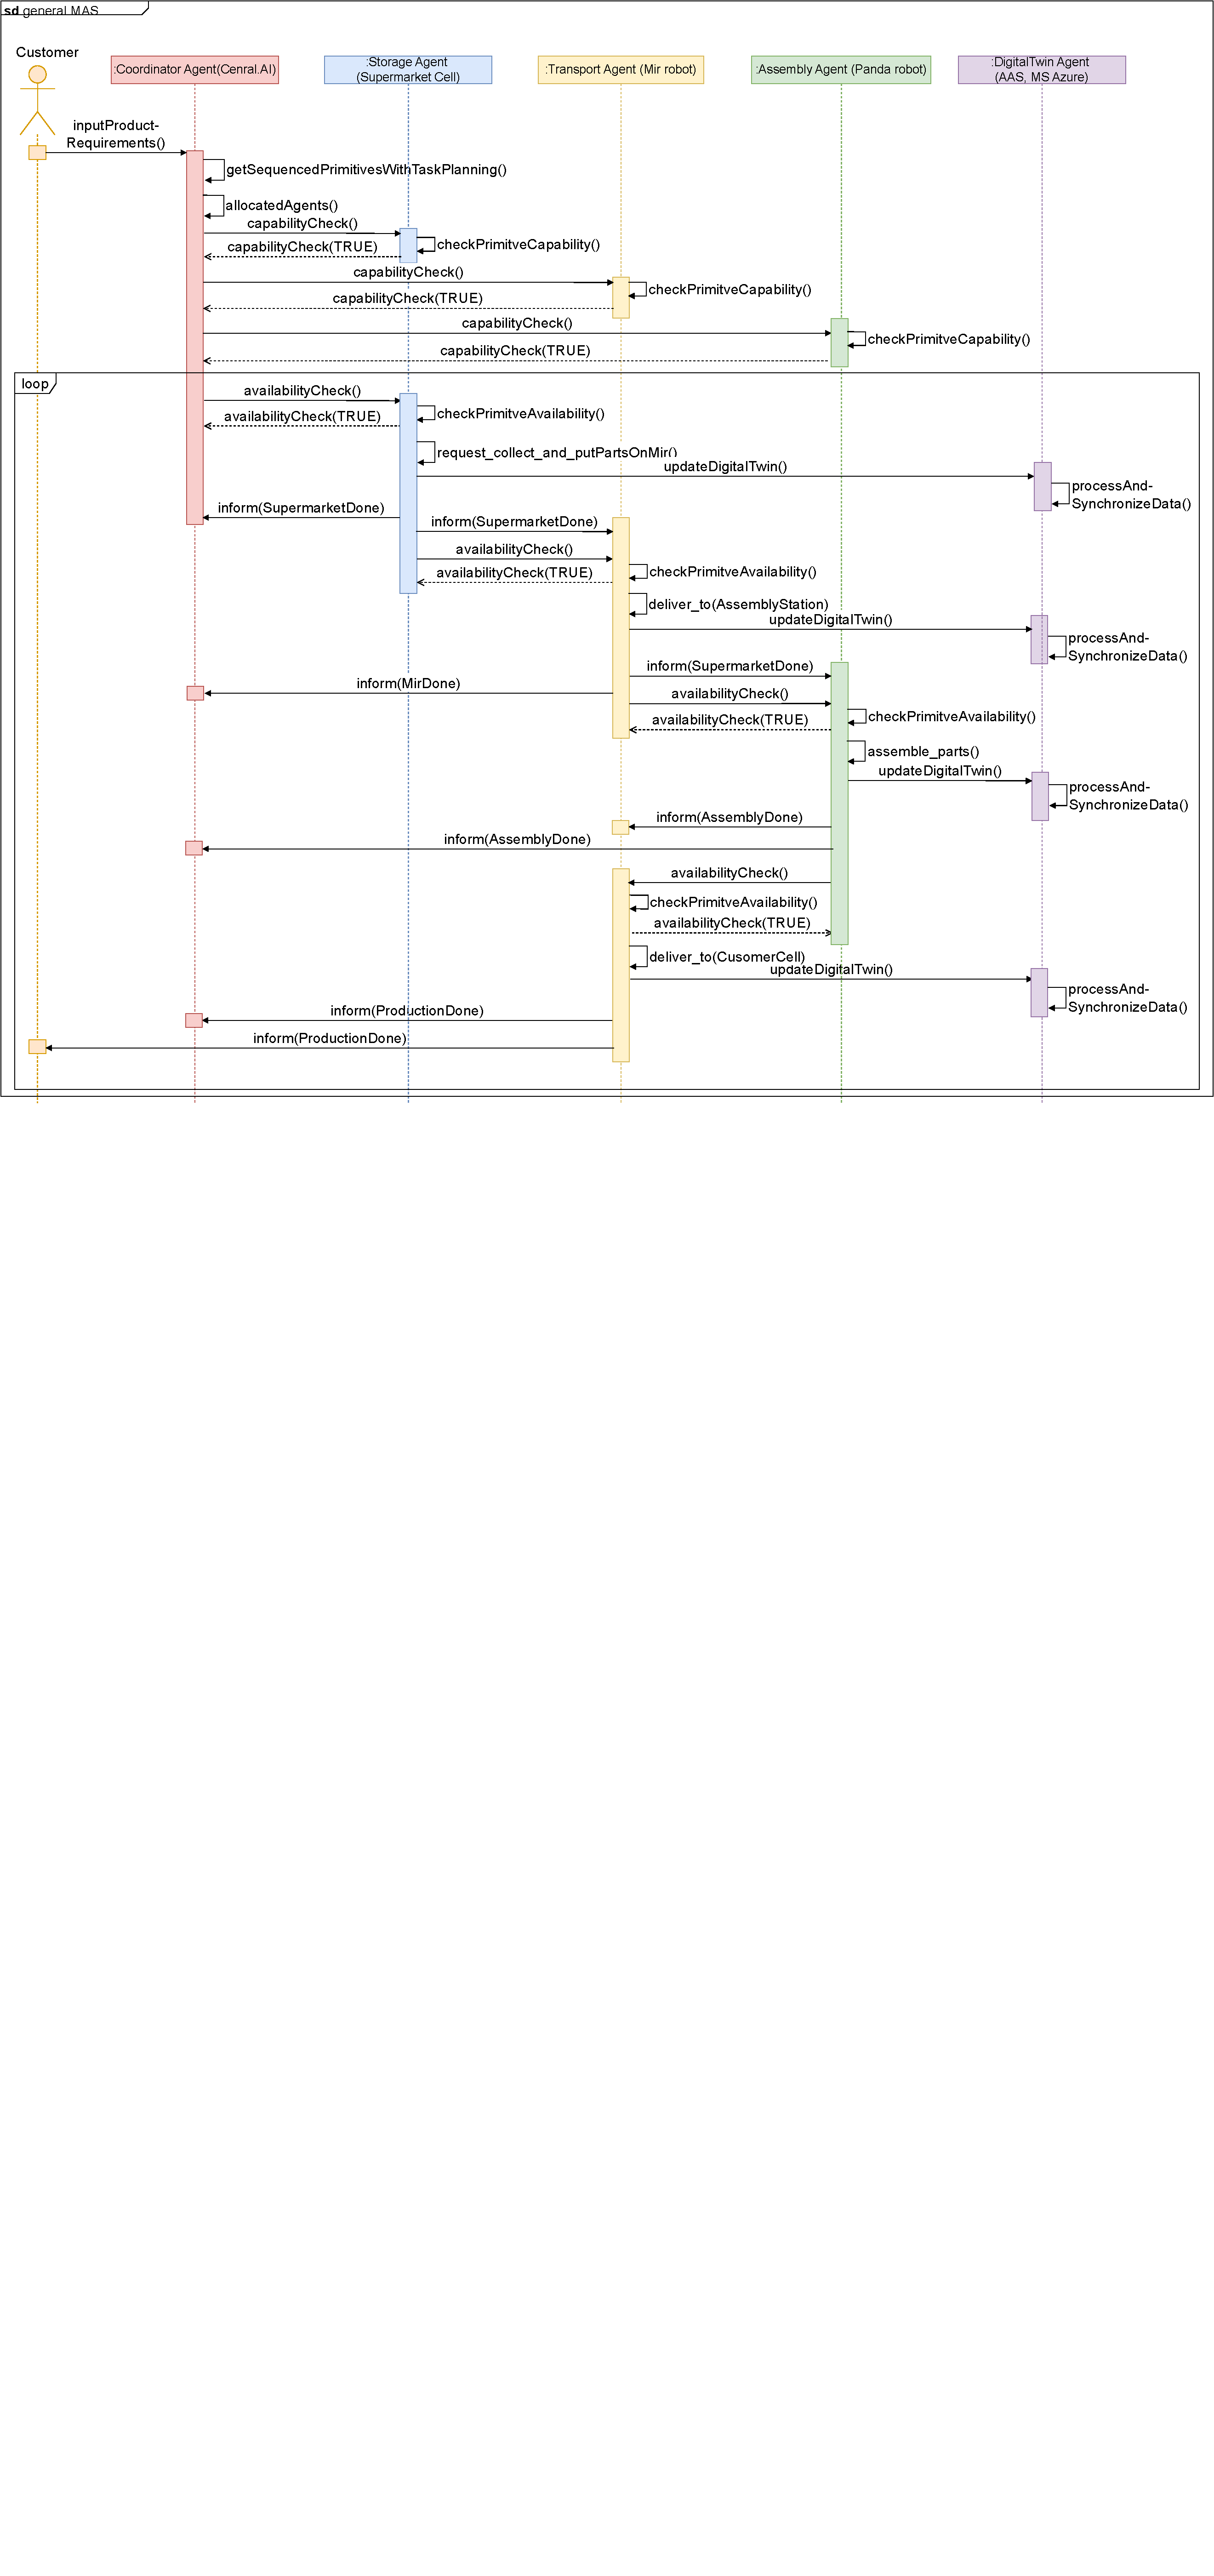
\includegraphics[width=\textwidth]{figures/tests/usecase/SequenceUsecases.pdf}\hfill 
    \caption{\gls{uml} general use case diagram of the \gls{mas} architecture.} 
    \label{fig: sequence-diagram}
\end{figure}


\begin{figure}[htb]
    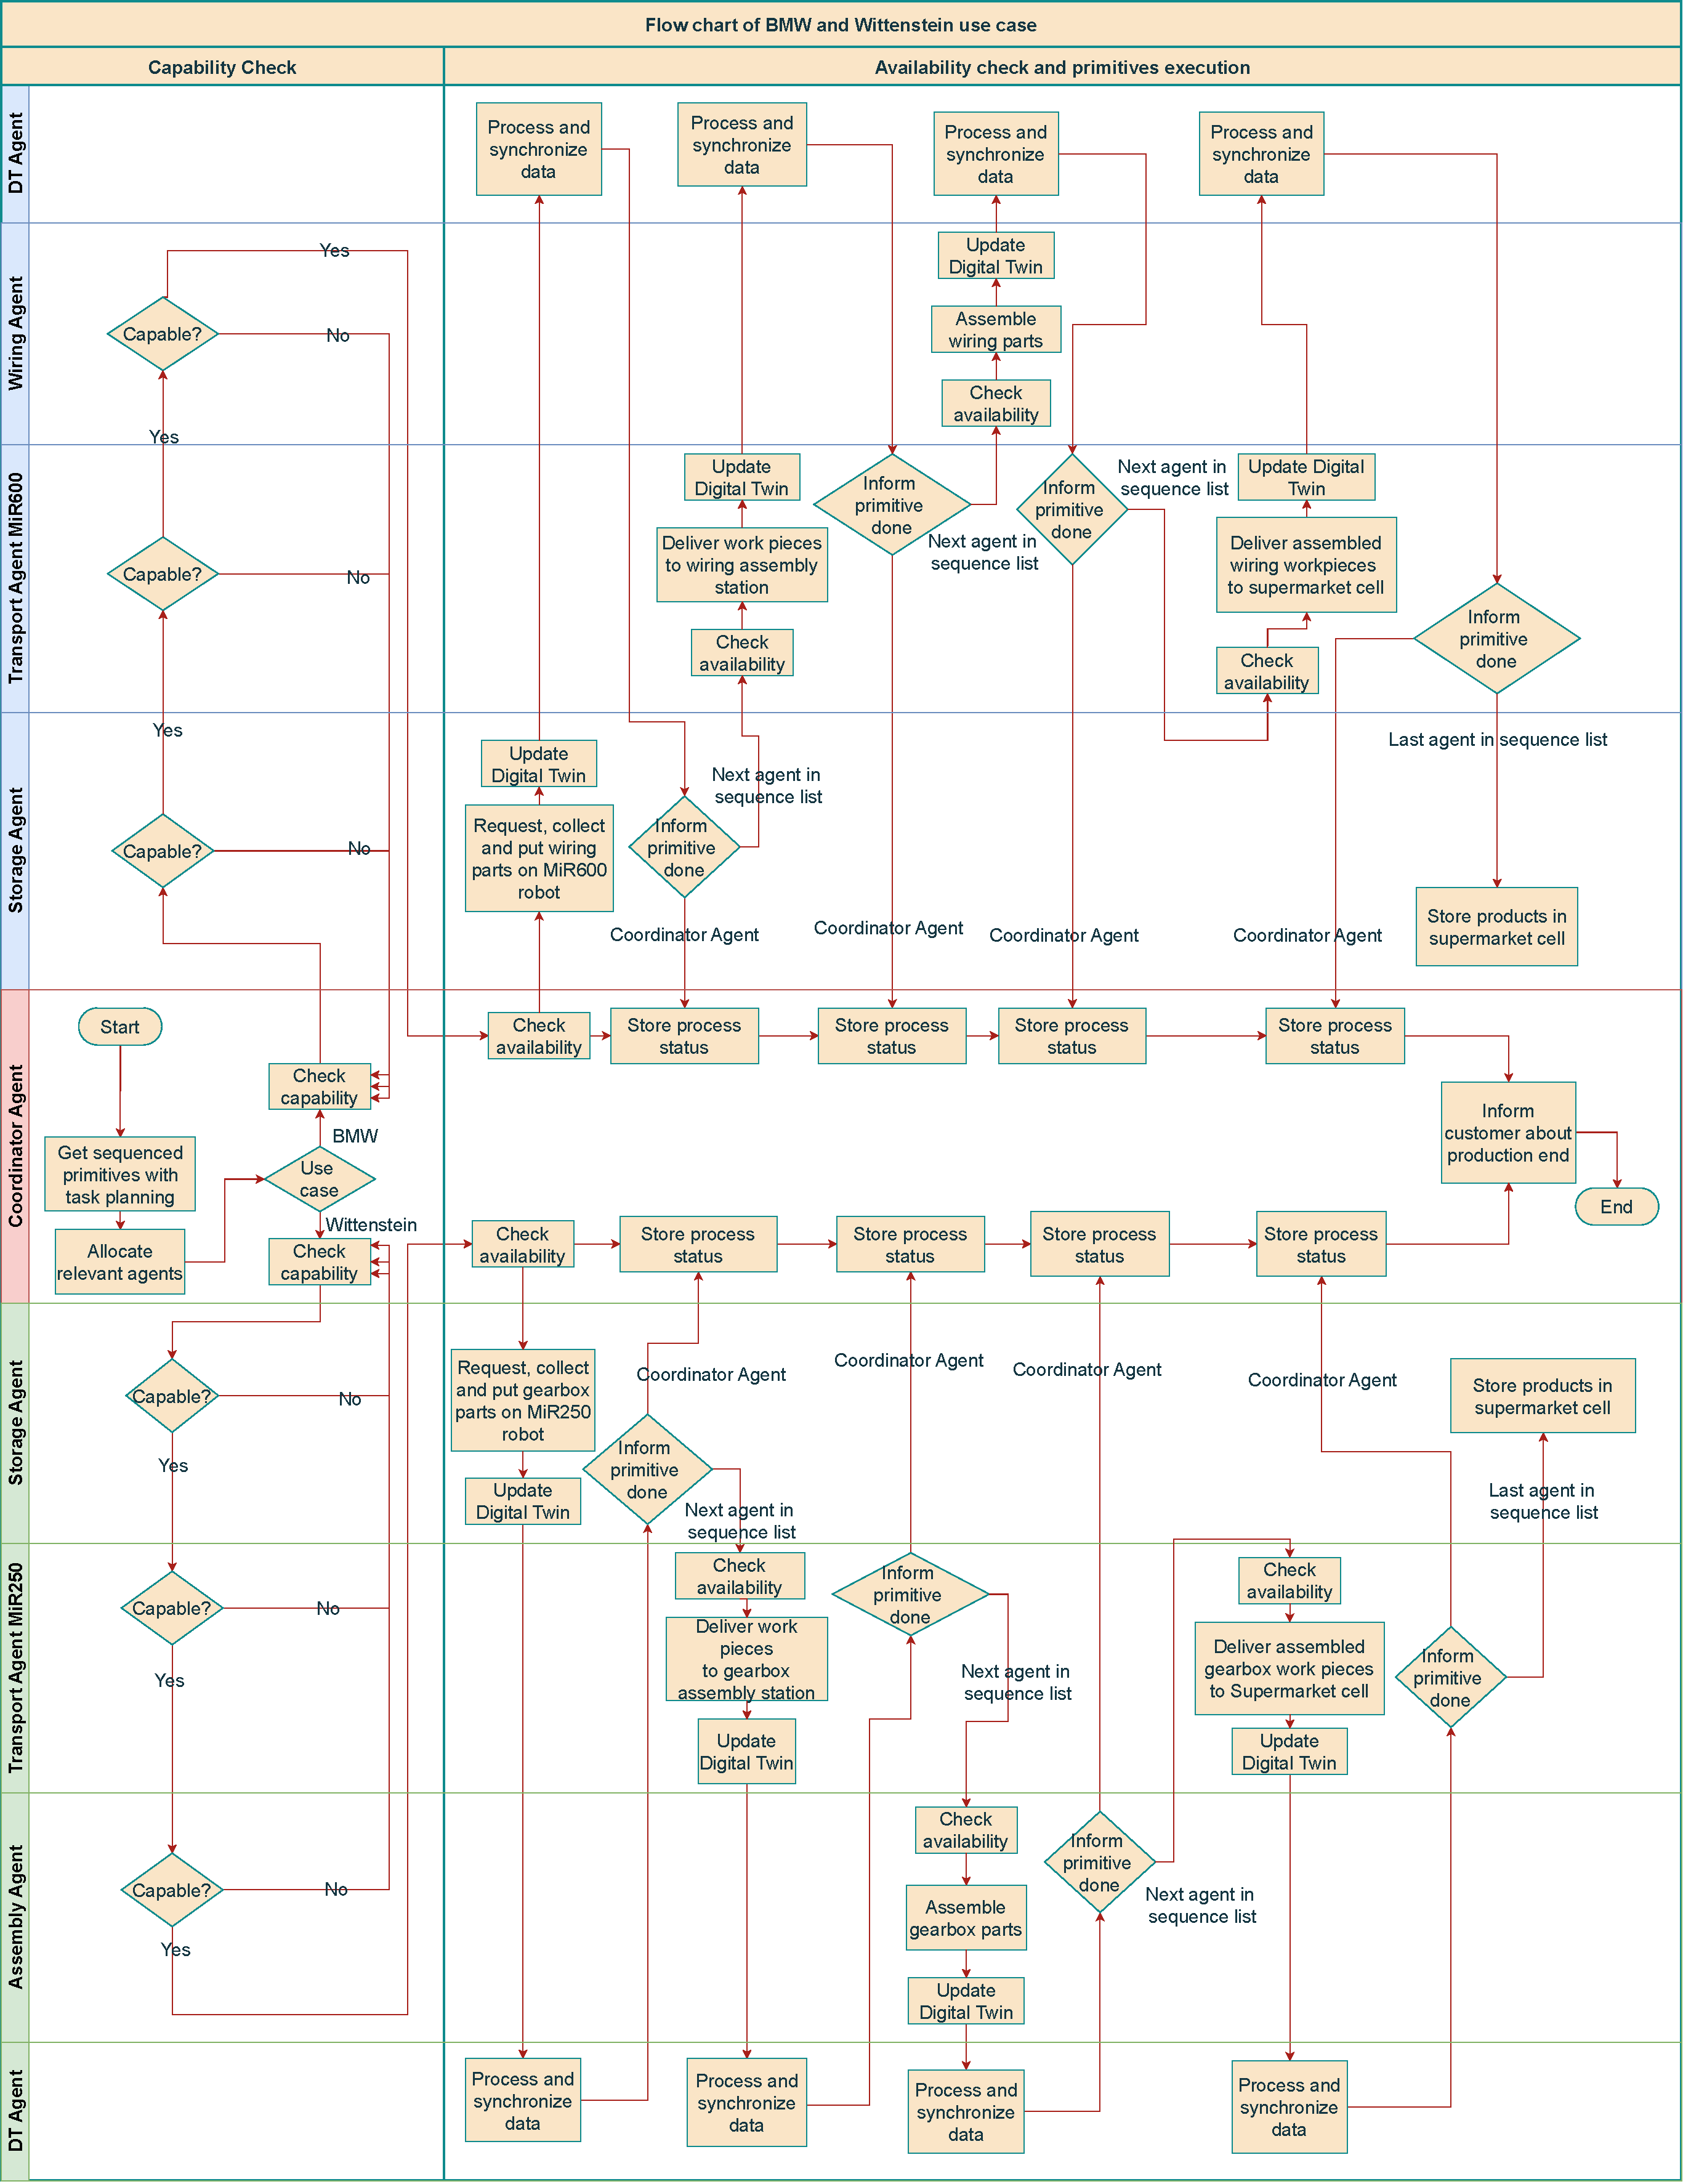
\includegraphics[width=\textwidth]{figures/tests/usecase/Usecase_flow.pdf}\hfill 
    \caption{Flowchart of BMW and Wittenstein use case of the \gls{mas} architecture. 
    Blue containers: BMW use case, allocated agents are Storge agent, 
    Transport agent MiR600, Wiring agent and Digital Twin agent respectively. 
    Green Containers: Wittenstein use case, allocated agents are Storage agent, 
    Transport agent MiR250, Assembly agent and Digital Twin agent respectively. 
    Red container: \gls{cda} for both usecases.} 
    \label{fig: Flowchart-usecase}
\end{figure}



For both BMW and Wittenstein use cases, the primitives with the associated agents and execution sequence are 
predefined. Although the program was designed based on two use cases, 
only the timing behaviors of the BMW use case was tested based on their similarity. 
The tab.\ref{tab: mean-usecase-time} shows the average \gls{rtt} and WebSocket 
data transmission time of BMW use case. The test was conducted a total of 100 times, 
but the number of messages 
each agent sent to the others during the test varied greatly. 
Due to the uneven amount of test data, 
the test results 
and average values can only be used as a reference to understand the data 
transmission process in actual production. A more detailed data ditribution of each 
message is presented as violin plot in fig.\ref{fig: violin-CDA-T600}. Together 
with the rest of the test results with other agents 
(see \ref{chap: append-UC} fig.\ref{fig: violin-CDA-ST} to \ref{fig: violin-T600-WI}), 
it can be concluded that 
the message transport in the system meets the real-time requirements, with the 
largest messge size of 636 Bytes in maximal 10ms and the smallest in about 0.2ms. 


\begin{table}[htbp]
    \small
    \centering
    \caption{Average delays between agents with different string message length and 
    different amount of messages.}
    \label{tab: mean-usecase-time}
    \begin{tabular}{|m{0.13\textwidth}|m{0.17\textwidth}|m{0.17\textwidth}|m{0.17\textwidth}|m{0.17\textwidth}|}
    \hline
    \multicolumn{5}{|c|}{\textbf{Average delays between agents (RTT/Transmission time)}}                                                            \\ \hline
    \textbf{}                         & \textbf{Coordinator Agent}             & \textbf{Storage Agent}        & \textbf{Transport Agent MiR600}    & \textbf{Wiring Agent}\\ \hline
    \textbf{Coordinator Agent}      & None                  & 1.029355ms /0.820172ms & 1.067170ms /0.849335ms  & 1.032151ms /0.817049ms \\ \hline
    \textbf{Storage Agent}          & 0.998253ms /0.794590ms & None                  & 1.427890ms /1.158142ms  & None                  \\ \hline
    \textbf{Transport Agent MiR600} & 1.055389ms /0.840291ms & 1.422970ms /1.150696ms & None                   & 1.668750ms /1.344250ms \\ \hline
    \textbf{Wiring Agent}           & 0.988012ms /0.783014ms & None                  & 1.654000ms /1.361000ms  & None                  \\ \hline
    \end{tabular}
\end{table}


\begin{figure}[htb]
    \centering
    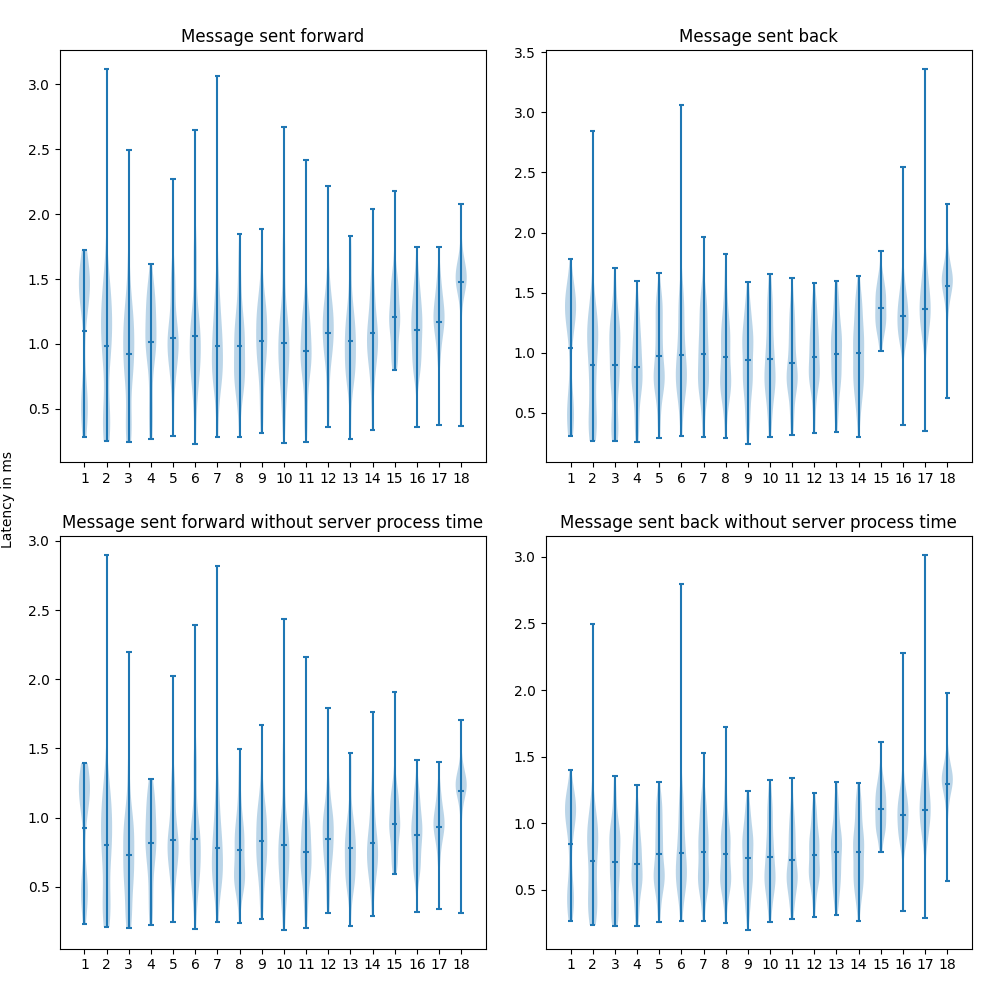
\includegraphics[width=\textwidth]{figures/tests/usecase/violin_CoordinatorAgent_to_TransportAgent_MiR600.png}\hfill 
    \caption{Test to measure \gls{rtt} and transmission time between \gls{cda} and 
    TransportAgent\_MiR600 for 100 times. The number in x-axis respresents the 
    corresonding messages. \protect\ref{firstfootnote}}
    \label{fig: violin-CDA-T600}
\end{figure}

%addtional for footnote in caption
\footnotetext[1]{\label{firstfootnote}https://github.com/XuezhouHou/Websocket\_MAS/new\_MAS/output/plots/table4UCBMW.xlsx}



\section{External}\label{chap: Result-External}
As for the delay measurement of the external \gls{dta} system, tests for the 
upload and download are done separately, with different packet sizes as tuning 
parameters. 


\subsection{Test results of data transmission time in \gls{tcp} sockets between robots and \gls{dta} 
in different packet lengths} \label{chap: Result-RCP-DTA}

To better measure the influence of different packet lengths on transmission time from 
a \gls{rcp} to \gls{dta} utilizing 
\gls{tcp} sockets, 
the packet length of JointGripper (joint and gripper of the robot arm) position values should 
be larger than that of the Elbow (elbow of the robot arm), they are 151 and 80 Bytes respectively. 
As depicted in 
fig.\ref{fig: SR-JointGripper-Elbow}, the mean transmission time of JointGripper is larger 
than Elbow, which verifies that larger files take longer to transfer. The cumulative delays of 
both data lengths also show a linear growth relationship 
in the upper graph, which means, there are no major fluctuations or irregularities 
in transmission speeds or times for the packets in \gls{tcp} sockets. 


\begin{figure}[htb]
    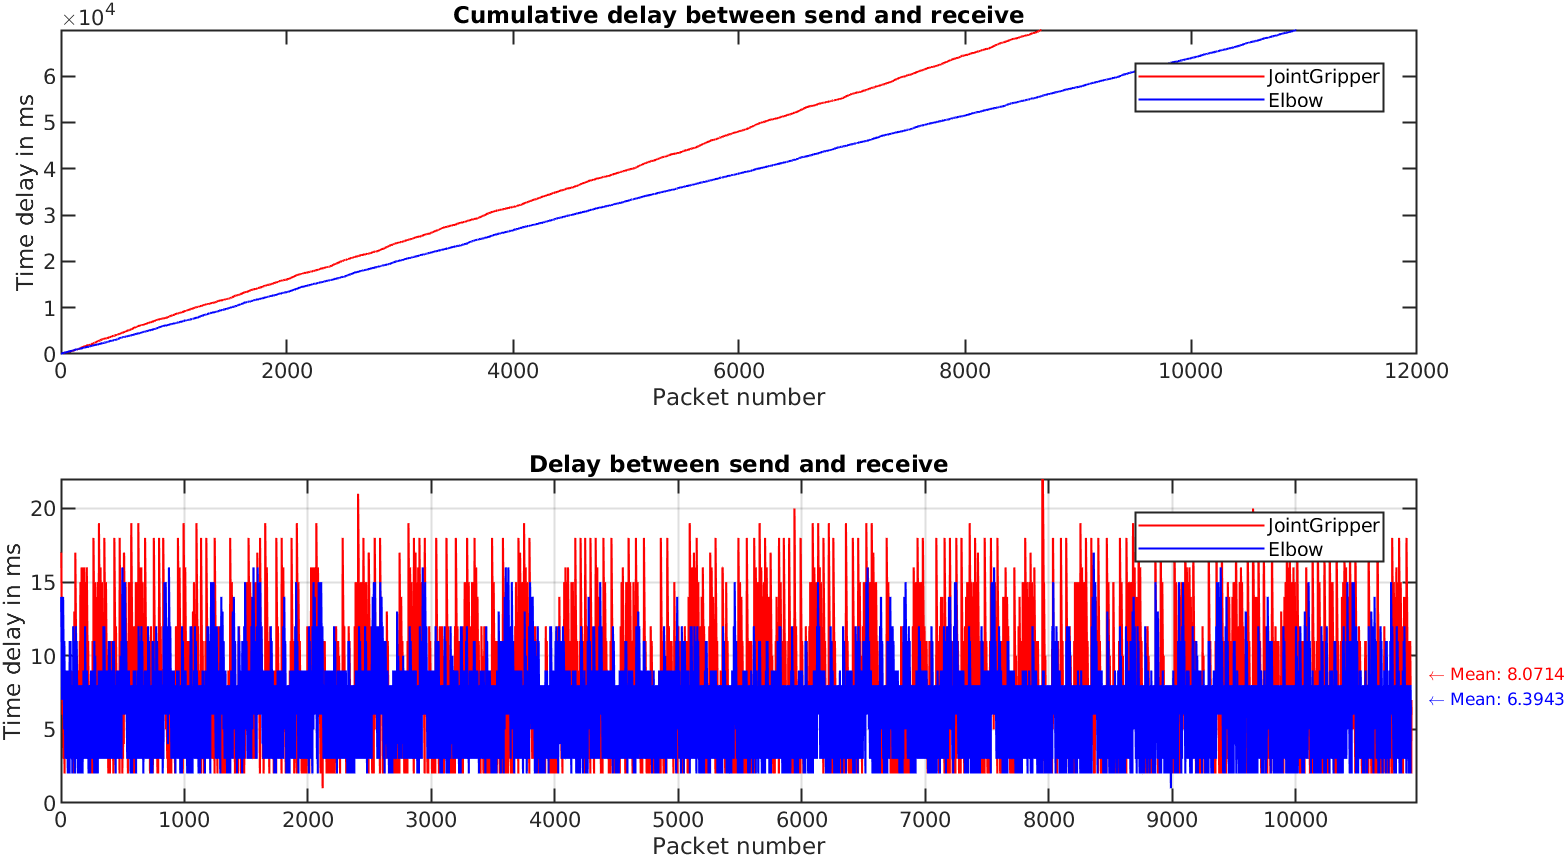
\includegraphics[width=\textwidth]{figures/tests/DT/Delay_SendReceive_JointGripper_Elbow.png}
    \centering
    \caption{Tests for different packet sizes w.r.t data transmission time between robots 
    and \gls{dta}. \label{fig: SR-JointGripper-Elbow}}
\end{figure}

Since each packet only takes a few milliseconds to be transported, the real time requirement 
for production processes is again fullfilled. 



\subsection{Test results of data transmission time in \gls{tcp} sockets between \gls{dta} 
and \gls{ms} Azure Digital Twin Cloud in different packet lengths} \label{chap: Result-DTA-DT}

However, in the program, the biggest variance 
on the total data transmission time is the \gls{rtt} from local devices to the global digital 
twin. In addtion to the \gls{rtt}, the data upload and download time is also measured 
separately, which has an opposite result as those from the other research\cite{cainelli_performance_2023}. 
In the paper, the resulting uplink data transmission time is larger than the downlink data transmission 
time. The difference between both tests is, the research team from Magdeburg 
measured delay with logical links from a 5G standalone network and the industrial 5G devices, 
whereas our test was based on data update times in the cloud. The latency 
between data upload and update reflects the actual digital twin data update 
patterns which includes additional process time in the cloud. Therefore we can 
infer that the increased latency of data upload may be caused by the internal 
Azure Digital Twin Model API for data update 
(unclosed issue in \gls{ms} Q\&A\footnote{https://learn.microsoft.com/en-us/answers/questions/1328803/experiencing-slow-load-times-on-azure-digital-twin}).
    

It is worth mentioning that the data upload time from JointGripper and Elbow 
has little to no difference, since the upload mechanism of Azure Digital Twin is limited 
by sending twin values one after one. There is no such function to update more than 
one twin simultaneously. In order to differentiate the upload speed, the patch size 
of the to be updated twin values should vary. The fig.\ref{fig: UD-cycle-JointGripper} 
again shows the cumulative delays with the same conclusion as in 
fig.\ref{fig: SR-JointGripper-Elbow} and mean \gls{rtt} is slightly lower than 
100ms, which is still under the real time requirements. As the packet for upload 
and download will be routed to the cloud, which not only goes through 
the internal 5G network but also the internet externally, which results in a much 
higher latency. Compared with the tests results from \cite{cainelli_performance_2023}, 
the internal twin update mechanisms can be optimized to further reduce the data 
upload and download \gls{rtt}. 


\begin{figure}[htb]
    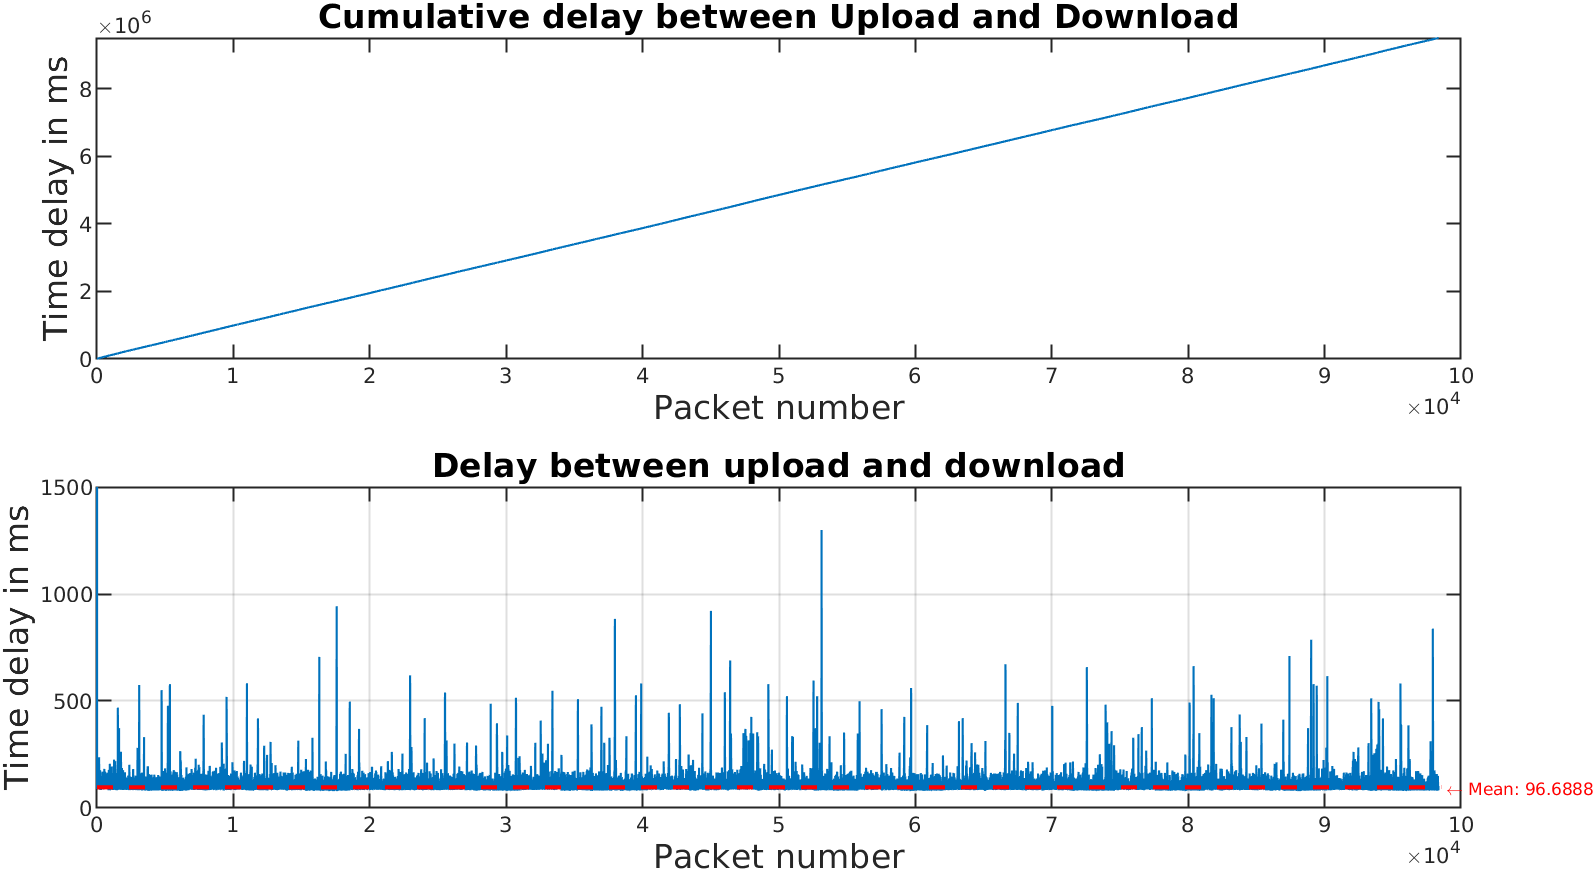
\includegraphics[width=\textwidth]{figures/tests/DT/Delay_UploadDownloadCycleTime_JointGripper.png}
    \centering
    \caption{Tests for \gls{rtt} of data upload and download for JointGripper. \label{fig: UD-cycle-JointGripper}}
\end{figure}

As mentioned, the data upload time is larger than the download time as depicted in 
fig.\ref{fig: UD-sep-JointGripper}. The upload time of JointGripper values is 
under 30ms while the download time results in about 70ms. Under the same conditions, 
the differences of both values for Elbow are negligible with 
only 1-2ms difference(see \ref{chap: append-DTagent} fig.\ref{fig: UD-cycle-Elbow} and 
\ref{fig: UD-sep-Elbow}), due to the one after one twin upload mechanism. 




\begin{figure}[htb]
    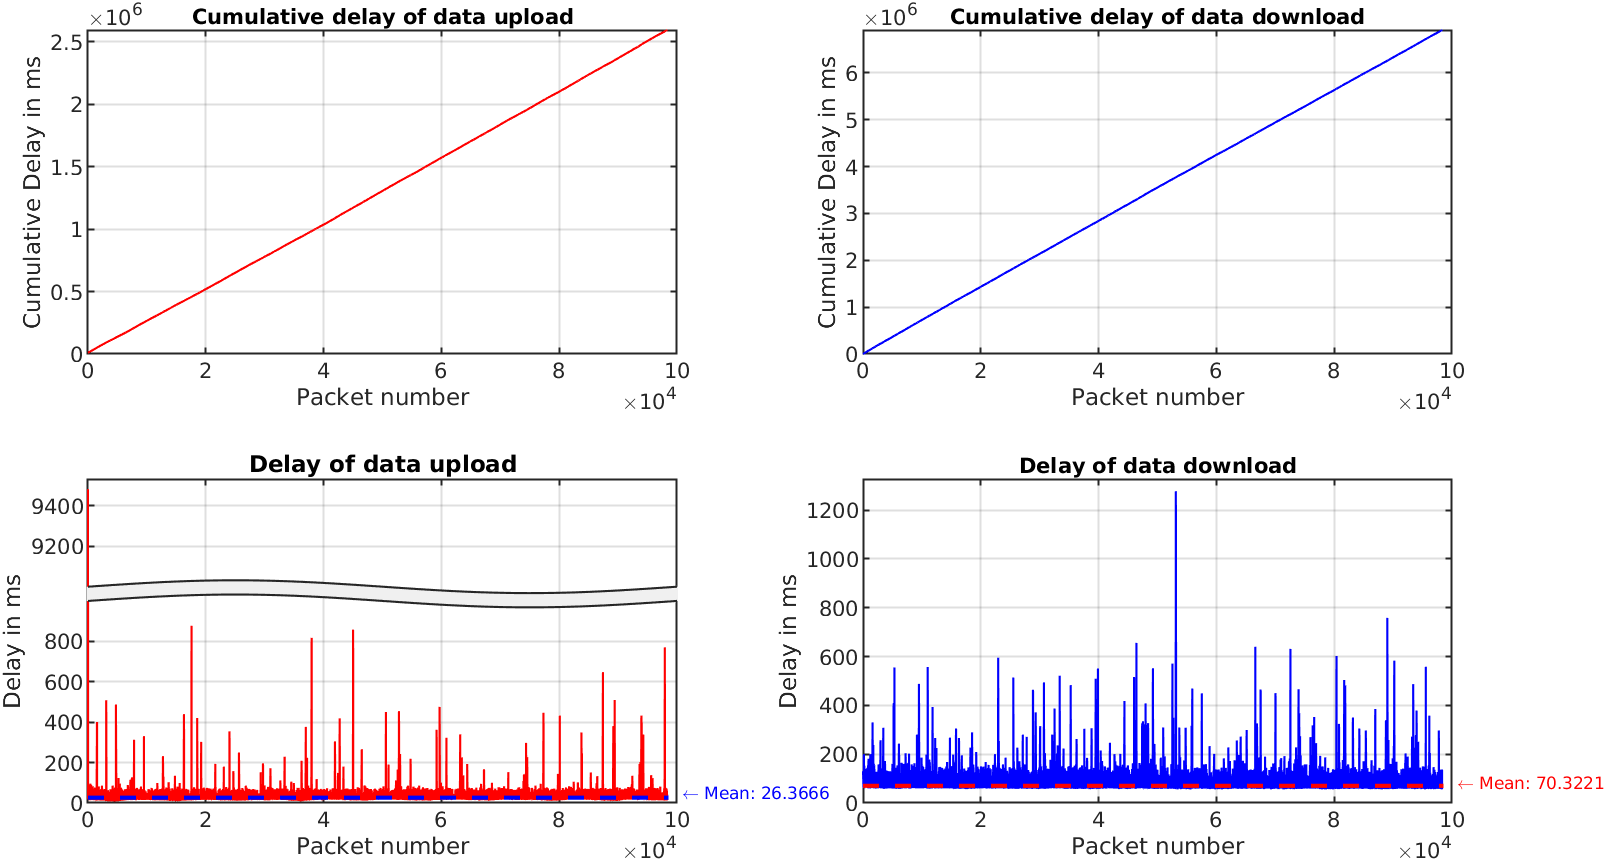
\includegraphics[width=\textwidth]{figures/tests/DT/Delay_UploadDownload_JointGripper.png}
    \centering
    \caption{Tests for delays between \gls{dta} and digital twin update of JointGripper, 
    and delays for twin value download. \label{fig: UD-sep-JointGripper}}
\end{figure}


To differentiate the upload speed based on packet size, two patches with 
different sizes are introduced. Ideally, the small data patch with a size of 
49 Bytes should induce a higher transmission speed than the large one with 
554 Bytes, but the reality is quite different. The test results of all the 
delay measurement for both patch sizes are presented as a violin plot in 
fig.\ref{fig: UD-violin-patchsize}. As expected, the upload time of large 
patches is less than small patches, while the result of download time is the 
opposite. This results to a almost identical total \gls{rtt} of both. 
The reasons can be, that each test is done at different time, which results in 
a fluctuation related to the network traffic, cloud service loads, amount of 
end users under the same 5G network and many more, which influence the data transmission 
time even more than the patch sizes.

\begin{figure}[htb]
    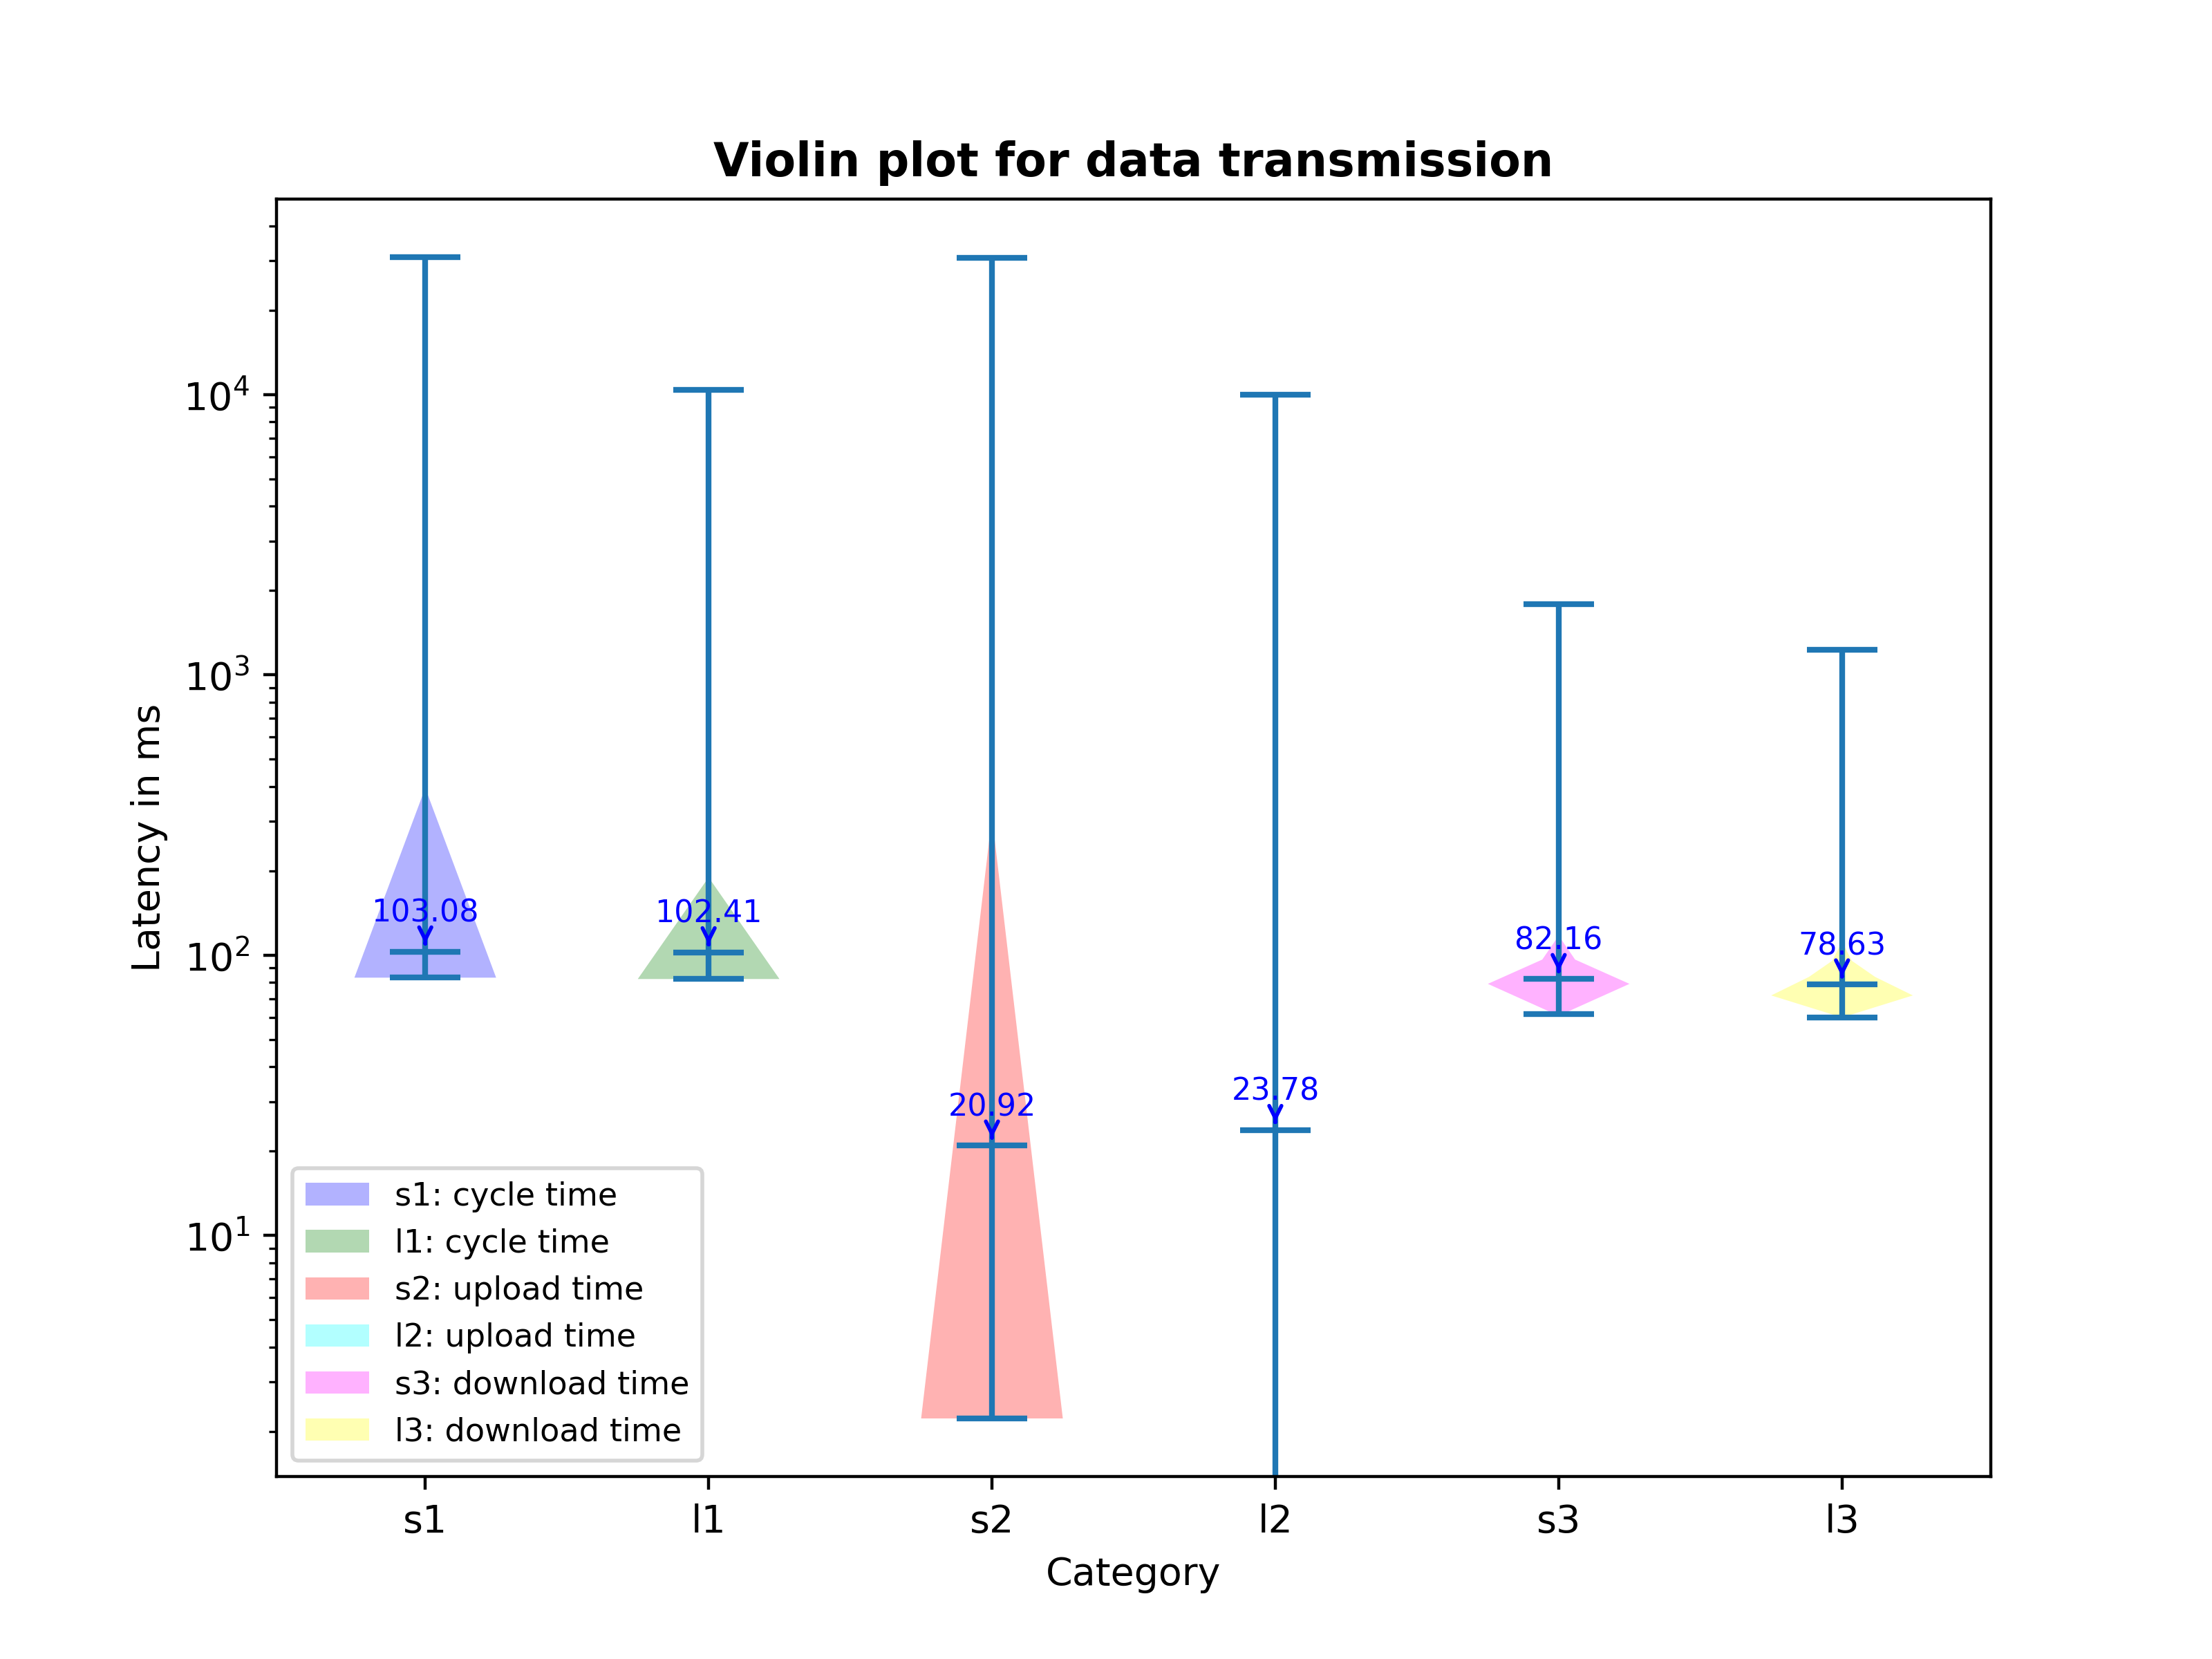
\includegraphics[width=\textwidth]{figures/tests/DT/violin_patch_size.png}
    \centering
    \caption{Tests for \gls{rtt}, delays between \gls{dta} and digital twin 
    update of JointGripper, and delays of twin value download for 
    two different patch sizes. In the graph, s represents small patches 
    and l for large patches.\label{fig: UD-violin-patchsize}}
\end{figure}

In genral, the data upload and download time between \gls{dta} and the cloud 
is much higher than the field 
level data transmission time under \gls{tcp} sockets. A fig.\ref{fig: SR-U-D-violin} shows 
the variance and mean of those in a violin plot for a more intuitive observation. 
Compared to the violin plot in fig.\ref{fig: UD-violin-patchsize}, the send and receive 
processes always show a symmetric triangular shape, suggesting a limited sample size. 
Considering the non-symmetric triangular shape of 
the uploading and downloading processes, 
this is likely be attributed to the data points with a predominance at the lower extremum, 
and the minimal presence at the upper extremum.
\begin{figure}[htb]
    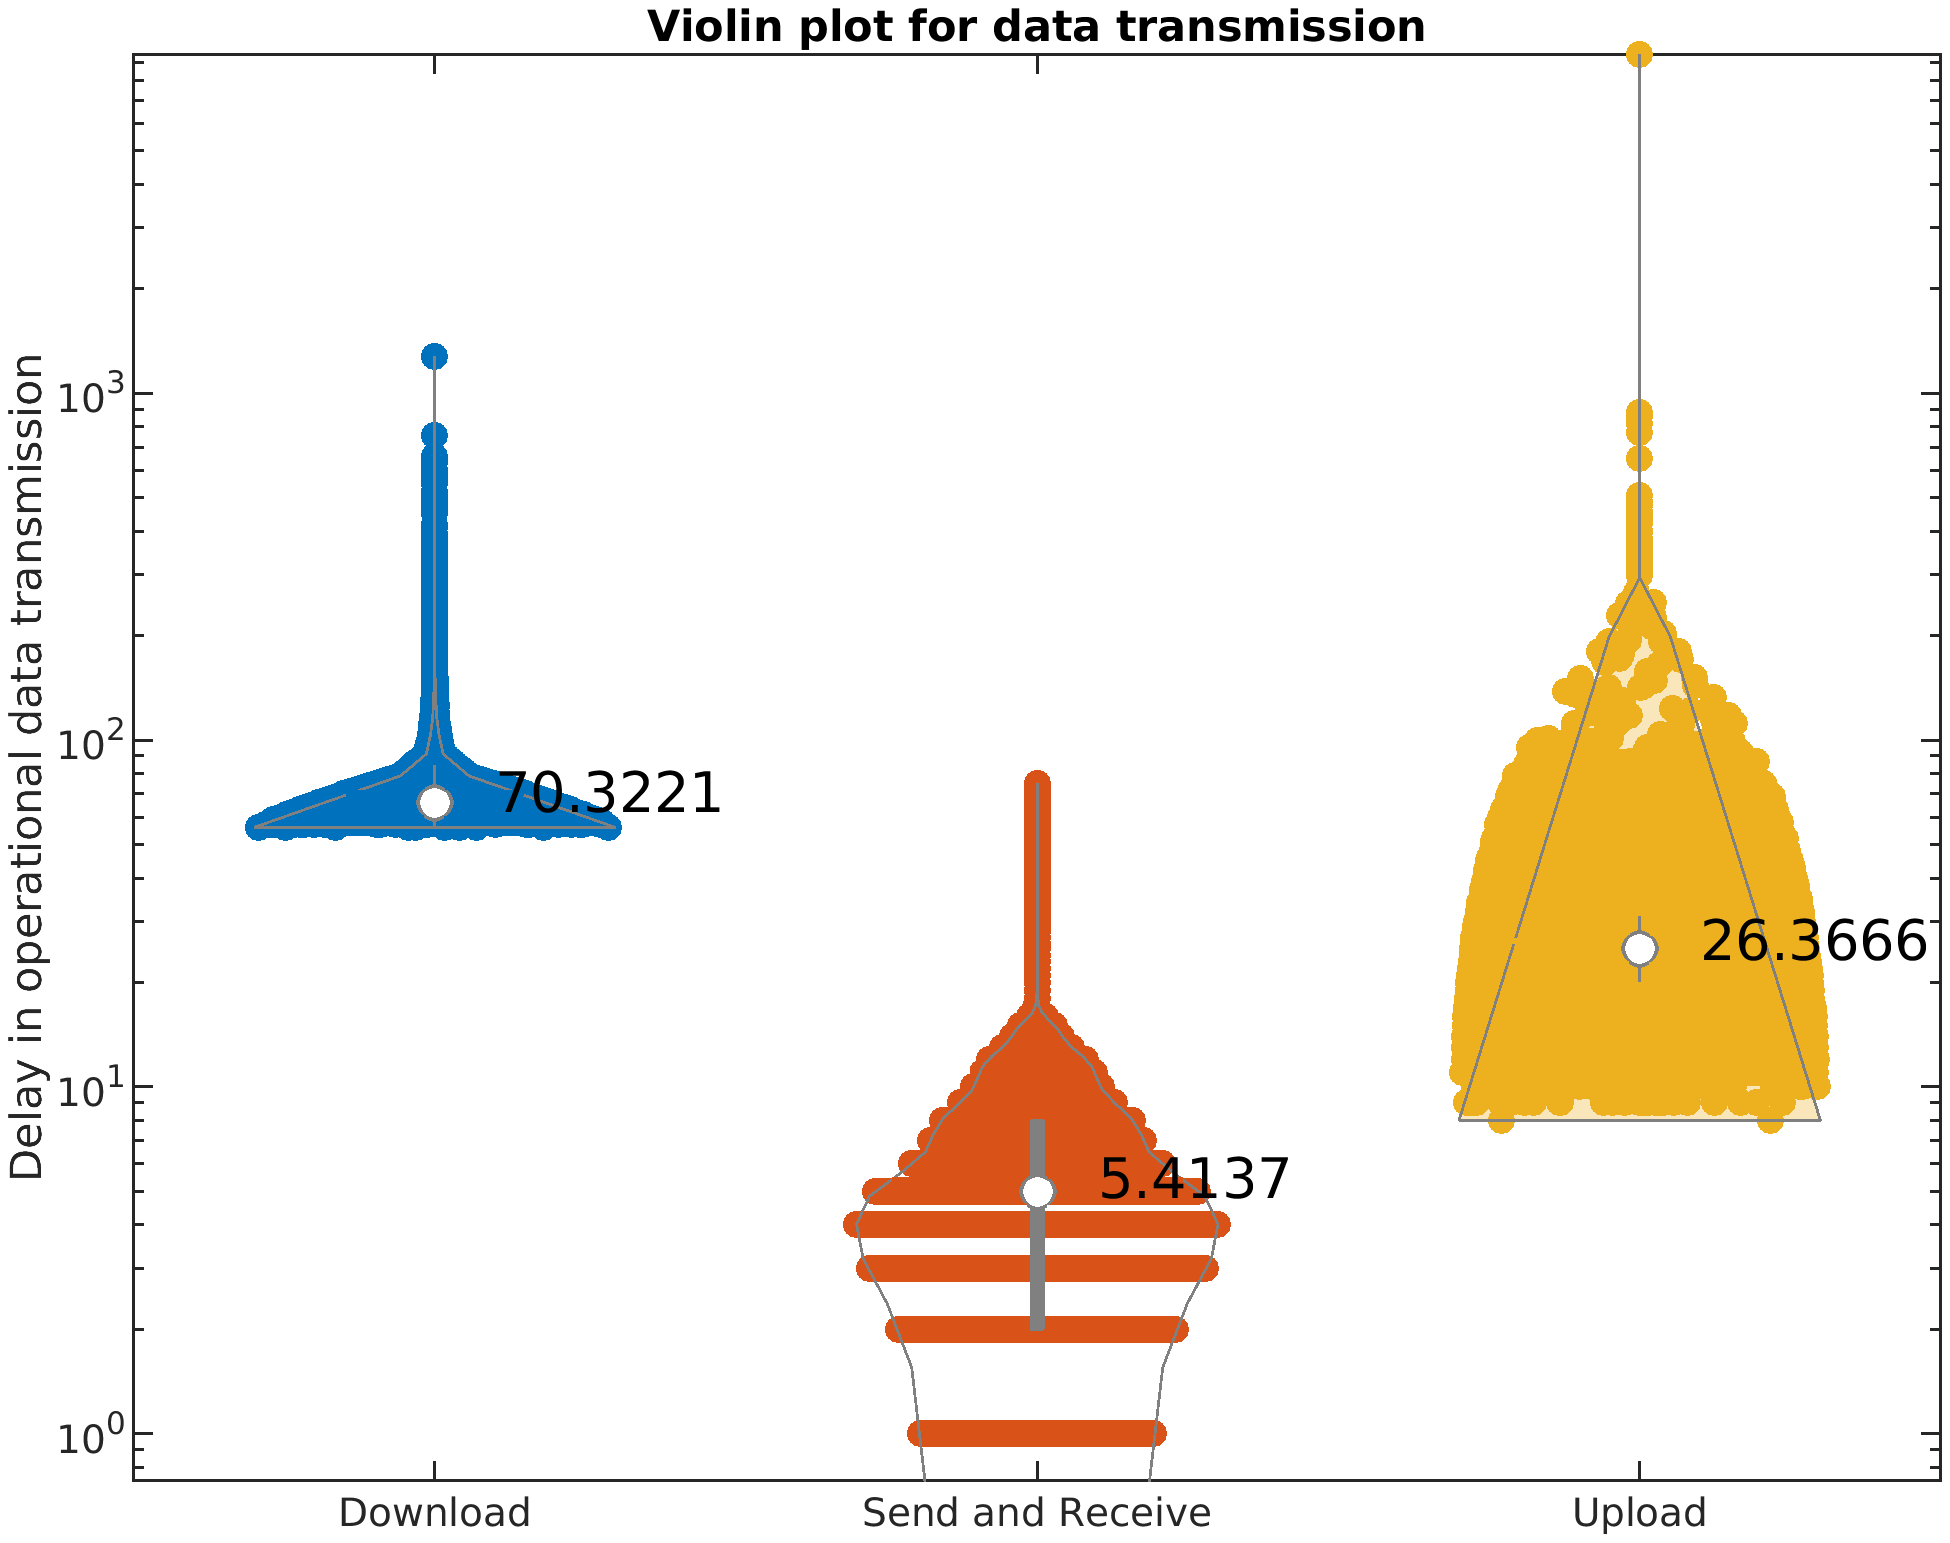
\includegraphics[width=\textwidth]{figures/tests/DT/log_violin_Plot_3cat.png}
    \centering
    \caption{Tests for data transmission time from robot to \gls{dta}, 
    delays between \gls{dta} and digital twin 
    update of JointGripper, and delays for twin value download.\label{fig: SR-U-D-violin}} 
\end{figure}

